\begin{justify}
\chapter[Resultados]{Resultados}
\label{ch:resul}
En este capítulo, se presentarán los aportes en el desarrollo del modelo de simulación, como también en el módulo de transición entre IPv6/LoRaWAN. Adicionalmente se entregarán los resultados obtenidos de las mediciones realizadas en la transmisión de nodos LoRa tanto en el ambiente virtual como en el empírico, esto acompañado de el análisis de los resultados, de las anomalías presentes, de los obstáculos que se presentaron en el desarrollo de estas pruebas y como ésto afectó a los resultados.

\section{Definición de variables y parámetros}
\label{sec:param}
Para el desarrollo del modelo de simulación es necesario acotar el sistema a simular, a los objetivos centrales del proyecto, para así evitar perder el foco deseado por realizar un modelo complejo, es decir, evitar realizar un modelo que incluya de forma innecesaria, variables que no generan un impacto tal en las mediciones, que merme la sensibilidad del modelo de simulación por sobre el nivel tolerado (\SI{3}{\percent}). Dado que el fin de esta simulación es imitar el comportamiento físico de los dispositivos LoRa, algunos datos que en condiciones reales son variables serán tomadas como parámetros estáticos con el fin de simplificar el modelo de simulación. Los valores asignados a estas variables, fueron obtenidos en la guía del desarrollador para dispositivos LoRa de la empresa Orange~\cite{orange}. Estos datos son escogidos dado que múltiples investigadores al realizar pruebas empíricas, usaron estos mismos datos como base para sus investigaciones con los dispositivos LoRa, obteniendo resultados muy cercanos a los que entrega la especificación de LoRa~\cite{Juha}. Los parámetros constantes de este sistema a modelar son los siguientes:
\begin{itemize}
\item Tasa de codificación=$\frac{4}{5}$
\item Ancho de Banda=\SI{125}{\kilo\hertz}
\item \gls{per}=\SI{1}{\percent}
\item Tasa de envío de datos en \textit{gateway} inicial=\SI{300}{bps}
\label{para:1}
\end{itemize}
\noindent
En relación a los parámetros fijos para el modelo de simulación, se aprecia en Tab~\ref{tab:par}, que se han definido valores fijos para variables dependientes de los \gls{sf} (tasa de envío de datos, alcance de transmisión, \textit{Time on Air}) a usar en la etapa de \gls{adr} de la comunicación LoRa~\cite{orange}.
\begin{table}[!ht]
\centering
\begin{tabular}{|c|c|c|c|}
\hline
\gls{sf} & bit rate & Alcance de Transmisión & \textit{Time on Air}\\ \hline
SF7 & $5470bps$ & $2km$ & $56ms$ \\ \hline
SF8 & $3126bps$ & $4km$ & $100ms$ \\ \hline
SF9 & $1760bps$ & $6km$ & $200ms$ \\ \hline
SF10 & $980bps$ & $8km$ & $370ms$ \\ \hline
SF11 & $440bps$ & $11km$ & $740ms$ \\ \hline
SF12 & $290bps$ & $14km$ & $1400ms$ \\ 
\hline
\end{tabular}
\caption{Asignación de valores para los diferentes \glsentryname{sf}.}
\label{tab:par}
\end{table}
\subsection{Arquitectura de red}
Para la comunicación en una red LoRa, se requiere una cantidad mínima de componentes para lograr la comunicación efectiva entre los dispositivos. Estos componentes mínimos para la comunicación son los siguientes:\\
\begin{itemize}
\item Concentrador LoRa (\textit{gateway})
\item Nodo LoRa
\item Micro computador conectado a Concentrador (\textit{backend})
\item Micro computador conectado a Nodo (\textit{backend})
\end{itemize}
Esta distribución mínima de componentes para asegurar la comunicación, puede verse en la Fig~\ref{lora:arc}. Esta arquitectura de red mínima se debe a que los dispositivos LoRa, sólo son provistos de las placas y antenas para el envío y recepción de paquetes en una red LoRa, pero no poseen la inteligencia para tomar decisiones o realizar acciones de forma autónoma, por lo que se requieren micro computadores (podría ser cualquier tipo de computador, pero se sugiere micro, para ahorrar consumo de energía) que le otorgue la inteligencia y sustente en energía a los dispositivos LoRa y a los sensores conectados a éstos. Adicionalmente, puede proveerse de un servidor que aloje una \gls{api} y una base de datos, con el fin de intercomunicar un servicio web, o para almacenar los datos censados en la red LoRa.\\
Para las pruebas realizadas en las mediciones de ambientes reales, se utilizó el esquema de arquitectura de red mínima, dado que al modelar los resultados obtenidos, tanto del funcionamiento lógico, como del funcionamiento físico, es posible proyectar estos resultados en arquitecturas de red a redes con un nivel mayor de complejidad, es decir, con un mayor número de elementos o distribuciones de éstos. Bajo este contexto, se realizaron pruebas representativas tanto para esta arquitectura mínima, como para un mayor número de nodos, gracias a la proyección que entrega el modelo de simulación.
\begin{figure}[!ht]
\centering
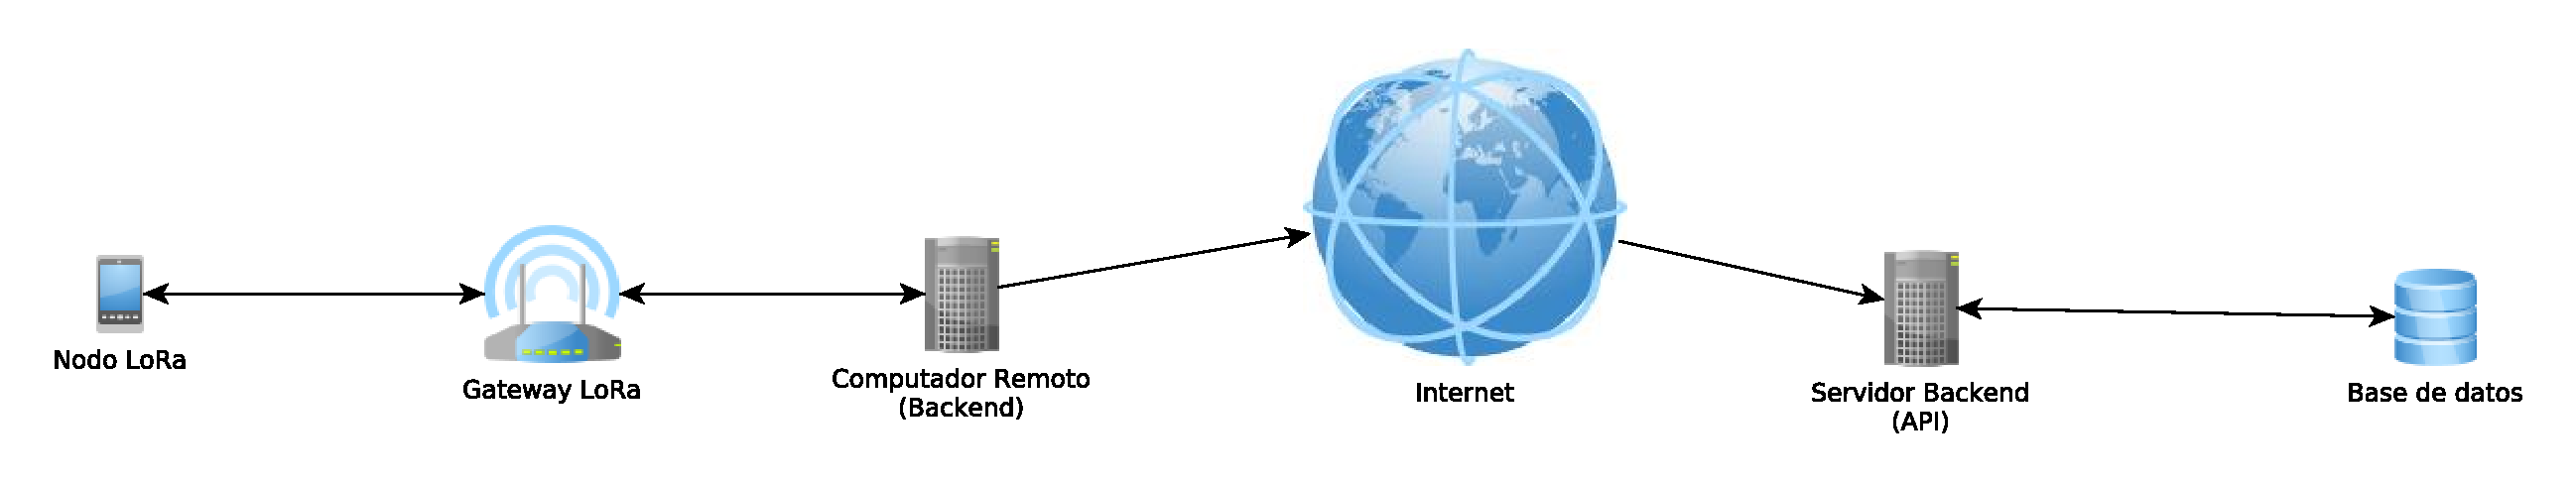
\includegraphics[scale=0.45]{diagramas/redminimalora.eps}
\caption{Diagrama de arquitectura de red mínima para una red LoRa}
\label{lora:arc}
\end{figure}
\newpage
\noindent
\section{Definición de fases de transmisión en LoraWAN}
Para que exista comunicación entre los nodos y \textit{gateway} LoRa deben ejecutar fases de comunicación, las que dan inicio a eventos, cómo el envío de un mensaje o el cambio de estado de un dispositivo. El identificar estas fases, para luego modelarlas, generará que el modelo de simulación sea más apegado al funcionamiento real de los dispositivos a simular. Dentro de las fases identificadas en la comunicación de los dispositivos LoRa se encuentran los siguientes:
\begin{itemize}
\item Fase de Emparejamiento
\item Fase de Transmisión
\begin{itemize}
\item[$\diamond$] Fase de Retransmisión (en caso de existir colisiones)
\end{itemize}
\item Fase de Reposo
\end{itemize}

\subsection{Fase de emparejamiento}
Durante esta fase, el nodo enviará un paquete \textit{Join Request} a todos los \textit{gateway} disponibles. Una vez que el \textit{gateway} reciba este mensaje, deberá responder dos mensaje de bajada que contendrán los identificadores de red, y dirección de la red LoRa para el nodo, adicionalmente se agregarán las llaves de sesión y aplicación en caso de que estén creadas.\\
Dado que en este modelo de simulación se busca sólo la simulación del comportamiento físico, los mensajes a programar en el modelo de simulación no poseen contenido alguno más que el nombre del mensaje que se está enviando, esto fue diseñado así para tener un mayor control en la depuración de la simulación y además para entregar un disparador de eventos de un objeto simulado al otro (nodo a \textit{gateway} y viceversa).\\
Los mensajes de bajada tendrán un desfase de envío de \SI{20}{\micro\s} más el tiempo que demora el paquete en llegar a destino, estos mensajes se identifican como \textit{Downlink-1} y \textit{Downlink-2}. \newpage \noindent 
Una vez que el nodo reciba estos mensajes, enviará dos mensaje \gls{ack}, pero luego de recibir los dos mensaje de bajada. En esta etapa, es donde internamente el nodo asigna todas las variables recibidas desde el \textit{gateway} para su correcto funcionamiento en la red.\\
Cuando el nodo envíe ambos mensajes de confirmación de los mensajes \textit{Downlink-1} y \textit{Downlink-2}, se asigna una variable distintiva (identificador de red y dirección de red LoRa) para evitar que un envío de datos sea rechazado por el \textit{gateway}, dado que en la simulación los mensajes no tendrán contenido, se asigna una variable tipo bandera, para distinguir a los nodos emparejados de los que no. Este fenómeno puede visualizarse en la Fig~\ref{pair:1}~\cite{Sornin}.
\begin{figure}[!ht]
\centering
\includegraphics[scale=0.5]{diagramas/pair}
\caption{Diagrama de flujo de mensajes para fase de emparejamiento en red LoRa}
\label{pair:1}
\end{figure}
\newpage
\noindent
\clearpage
\subsection{Fase de transmisión}

En el caso de que el nodo reciba bien ambos mensajes de bajada, como se observa en la Fig~\ref{trans:1}, se enviará un mensaje de petición de envío de datos (\textit{Uplink request}), a lo que en condiciones ideales (sin colisiones ni saturación de canal), el \textit{gateway} deberá responder con una confirmación de la petición de envío, deteniendo cualquier transmisión por aquel canal y quedando a la espera de la recepción del mensaje proveniente del nodo. El nodo una vez que recibe el paquete \gls{ack} de la petición de envío , este envía el paquete de datos al \textit{gateway}, donde en caso de no haber colisión, el \textit{gateway} respondería nuevamente con un paquete \gls{ack}, terminando con esto la fase de transmisión.\\


\begin{figure}[!ht]
\centering
\includegraphics[scale=0.6]{diagramas/transmit}
\caption{Diagrama de flujo de mensajes en fase de transmisión de paquetes en red LoRa}
\label{trans:1}
\end{figure}
\newpage
\subsubsection{Fase de retransmisión}
\justify
En el caso de que en cualquier fase ocurra una colisión o una interferencia que corrompa un bit en un paquete, el paquete será descartado y no llegará a destino, por lo que todos los dispositivos LoRa poseen un indicador de tiempo agotado (\textit{Timeout}) el que es igual a:
 
\begin{eqnarray}
 \textit{Timeout} [\SI{}{\milli\s}]= 2(\textit{Time on Air}) [\SI{}{\milli\s}]\end{eqnarray} \\
, donde \begin{eqnarray}
 \textit{Time on Air} [\SI{}{\milli\s}]= \frac{\textit{Largo del Paquete} }{\textit{Tx Data Rate}} \frac{[\SI{}{\bit}]}{[\SI{}{bps}]}\end{eqnarray}
\noindent
En la Fig~\ref{retrans:1} se describe el proceso lógico que realiza el simulador en caso de no recibir un paquete \gls{ack} luego de la petición de conexión, en el caso que el tiempo transcurrido sea mayor al valor de la variable \textit{Timeout}, el nodo volverá al estado previo de envío dependiendo si está pareado o no. En el caso de que se encuentre emparejado, volverá a la fase de transmisión para transmitir nuevamente el paquete \textit{Uplink-request} hasta que el \textit{gateway} le responda. Si el nodo no está emparejado, este volverá a la fase de emparejamiento donde enviará el paquete \textit{Pair-request}, hasta que el \textit{gateway} le responda con las dos ventanas de bajada (\textit{Downlink-1} y \textit{Downlink-2}).
\begin{figure}[!ht]
\centering
\includegraphics[scale=0.4]{diagramas/retrans}
\caption{Diagrama de estados que representa la fase de retransmisión}
\label{retrans:1}
\end{figure}
\subsection{Fase de reposo}
Luego de la transmisión del paquete \textit{Uplink-payload} desde el nodo al \textit{gateway}, si el \textit{gateway} contesta nuevamente con un último paquete de confirmación \gls{ack}, en este paquete el \textit{gateway} enviará los datos de su reloj interno para sincronizar y programar el próximo envío de datos, a lo que el nodo sincroniza su reloj interno y entra en un estado de reposo, a lo que no transmite ni recibe nada hasta que se cumpla la condición entregada por el \textit{gateway}. Este tiempo de reposo, es configurable desde el \textit{gateway}, con el comando MAC DutyCycleReq~\cite{Sornin}.
\subsection{Pérdida de paquetes}
Con el fin de acercar más a la realidad el modelo de simulación, se programó una función que simula la pérdida de paquetes en los distintos \gls{sf}, ésto lo realiza llevando una contabilidad de los mensajes recibidos, y genera una comparativa con el porcentaje de pérdida en la recepción donde se tienen tres condiciones principales. La primera es que el porcentaje de pérdida sea mayor que cero, y ésta debe ser siempre verdadera, dado que si fuera cero no debería entrar a la función que desechará paquetes. La segunda condición es una condición compuesta, donde debe cumplirse que el coeficiente entre el contador de recepciones con error, por el contador de envíos recibidos correctamente multiplicado por cien debe ser menor que el porcentaje de pérdida de paquetes, o en cambio es posible de que se cumpla de que el contador de errores sea igual a cero, con lo que también entraría a la función que desechará la recepción de datos.\\
Con esta función es posible emular un ambiente mas cercano al real, al poder incluir condiciones desfavorables en la simulación, como las que son posibles de encontrar en la vida real.

\section{Módulo de transición LoRaWAN/IPv6}
Para el desarrollo del módulo de transición de LoRaWAN a IPV6 se modificó el programa desarrollado por SemTech~\cite{script} para comunicar el \textit{gateway} con el nodo, generando un tipo de \textit{Middleware} entre la red LoRa y las redes externas a esta.\newpage \noindent
Gracias a modificaciones realizadas al script de SemTech, ahora es posible la obtención y visualización del \textit{payload} de forma íntegra y su retransmisión hacia redes externas a la red LoRa~\cite{tomas}.\\
En cuanto a llevar a cabo la retransmisión hacia redes externas de los paquetes LoRaWAN, hace falta generar una conexión puente que comparta salida a Internet al \textit{gateway} LoRa, esto se logra a través del uso de iptables u otro gestor de reglas de conexiones entrantes y salientes. Y luego mediante el uso de \glspl{socket} en C realizar la conexión hacia una base de datos o aplicación web, para luego procesar dichos datos y finalmente ser mostrados en algún front-end o servicio web.
\subsection{Funcionamiento}
El funcionamiento de este módulo es el siguiente, una vez que el \textit{gateway} ya posee la capacidad de escuchar, se debe lanzar un ping en IPv6 desde la Raspberry que posee de back-end. Una vez realizado esto comenzará una transmisión de paquetes donde se capturará el \textit{payload} del mensaje de LoRaWAN y se mostrará por pantalla,  ``Manda'' y ``LLega'' dependiendo si el mensaje llega de forma íntegra o no al \textit{gateway} (la cantidad de bytes especificada en la configuración, debe ser la misma cantidad de bytes que los contenidos en el struct array), en dicha parte del código se implementó un \gls{socket} en C para comunicarse con una base de datos MySQL creada para la interacción con este módulo, dado que si es posible comunicarse con la base de datos y realizar consultas a la base de datos (insert-delete-update) será posible la comunicación con casi cualquier servicio web que admita conexiones desde clientes.\\
En el extracto de código~\ref{anexc:1}, se presenta el código que maneja los métodos que permiten enviar datos como la IP del \textit{gateway} (obtenida mediante la implementación de IPv6 sobre LoRaWAN~\cite{tomas}), junto con el \textit{payload} a una base de datos, que en este caso sería una base de datos local. De esta forma se puede visualizar cómo es posible generar una capa intermedia de comunicaciones para el envío de datos entre la red LoRa y un servicio web deseado.
\subsection{Contribuciones}
Gracias a la contribución de la implementación de IPv6 en LoRaWAN, y a los mensajes de depuración del script para que imprima por pantalla los estados de los mensajes tanto salientes como entrantes (sólo los que llegan íntegros), es posible extraer el \textit{payload} de los mensajes enviados por los nodos hacia el \textit{gateway} para luego poder enviarlo hacia afuera para su almacenamiento en una base de datos, o para análisis de los datos en alguna aplicación sea web o móvil. Esto da la capacidad a una red LoRa de ejecutar comandos MAC, como también el extraer los datos hacia una aplicación que analice y cense los datos obtenidos, entre otros posibles usos~\cite{tomas}.
\subsection{Consideraciones}
Dados los problemas de conectividad presentes en los dispositivos físicos que se utilizaron durante la ejecución de las pruebas, tanto en el desarrollo del módulo como en las pruebas  de verificación, estas pudieron ser llevadas a cabo bajo la condición de poseer ambos dispositivos (Nodo y \textit{gateway}), a distancias muy cortas para maximizar la conectividad, dado que el objetivo de este módulo es probar la posibilidad de extraer datos de una red LoRa hacia Internet, y no el probar la capacidad de transmisión de los dispositivos físicos. Esto es mencionado dado que muchas veces los paquetes no llegan desde el nodo al \textit{gateway}, y no porque este no haya sido enviado, si no porque el \textit{gateway} lo detecta como mensaje, al analizar el campo MIC del paquete recibido, donde en el caso de que el \textit{hash} no coincida con el válido, se toma como paquete corrupto. Por lo que este módulo en esos casos no es capaz de enviar nada.
%%%PRUEBAS%%%%
\section{Parámetros y variables de mediciones}
Para verificar el funcionamiento del modelo de simulación de los dispositivos LoRa, se establecieron ciertos parámetros a medir, los que serán a posterior indicadores del buen o mal funcionamiento del modelo de simulación. Estos parámetros son, los cambios de estado de los dispositivos LoRa (en el caso del simulador), para verificar que está realizando todo el proceso de forma correcta. Además, se medirá el número de colisiones contra la cantidad de mensajes enviados y erróneos, para calcular el porcentaje de pérdida de paquetes estimado en cada prueba de transmisión. Estas pruebas se realizarán primero en el ambiente real, con el fin de obtener un valor estimado del porcentaje de pérdida de paquetes real, el que luego se aplicará al modelo simulado y será contrastado tanto entre el ambiente real, el ambiente virtual, como también contra los porcentajes de pérdida de paquetes obtenido investigaciones relacionadas~\cite{Juha}. Este contraste de resultados, es realizado ya que el modelo de simulación, es desarrollado en un principio en una condición ideal de transmisión, por lo que no es afectado por ninguna variable del ambiente (interferencia por otras señales, edificios, interferencia por fuentes de poder,etc.) lo que lo hace poco real y por tanto no fiable como modelo de simulación, por lo que el objeto de este contraste es volver más fiable el modelo, agregando condiciones presentes en la realidad, al canal de transmisión virtual.\\
Adicionalmente para las pruebas de simulación se dispuso una distribución específica de los nodos para cada canal o \gls{sf}, dicha distribución es posible de encontrar en la Tab~\ref{tab:prueba}, donde se mostrará que cantidad de nodos está asignado a cada \gls{sf}, y que distancia en metros se le asignó para temas de la simulación. Estos datos explican la distribución de hasta diez nodos, la cual para las pruebas de cien nodos fue repetida diez veces con el fin de mantener la misma distribución pareja de nodos. Cabe decir que la correspondencia entre la distancia desde los nodos hasta el \textit{gateway} con el \gls{sf} asignado, fue tomado de datos de los desarrolladores de LoRa~\cite{orange}.\\
En relación a las pruebas de cambio de estado, en la Tab~\ref{tab:estados} se muestran la correspondencia de cada valor numérico con cada estado de los nodos durante la simulación. Dentro de los estados disponibles para los nodos se encuentran los siguientes:
\begin{itemize}
\item IDLE: Este estado es el inicial para cada nodo en la red, es el encargado de enviar el \textit{Pair request} al \textit{gateway} y luego quedarse a la espera de recibir las dos ventanas de descarga desde el \textit{gateway}.
\item PRERECEIVE: Este estado, sólo se encarga de esperar hasta que el \textit{gateway} envíe ambas ventanas de descarga, donde al llegar éstas y si el nodo no esta emparejado, envía la orden de cambiar a estado TRANSMIT.
\item TRANSMIT: Este estado es activado al recibir las ventanas de descarga. Es el estado que genera los mensajes \textit{Downlink-1-ack} y \textit{Downlink-2-ack}, los que serán enviados al \textit{gateway} para certificar de que se recibió la información de estos paquetes, los que en el caso de un emparejamiento real tendría relación con los identificadores de red, identificadores de aplicación y los tiempos que debe esperar entre cada ventana de subida de información.
\item RECEIVE: En este estado, se envía el primer \gls{ack} correspondiente a la primera ventana de descarga. Este estado, da paso directo al estado RECEIVE2, dado que la diferencia de recepción de envío de la primera y segunda ventana, es poca en comparación con el resto de mensajes (más o menos \SI{20}{\micro\s}, ésto permite la correcta recepción de ambos mensajes, sin pérdida del primero, o falla de sincronización en la fase de emparejamiento por un sobre encolado de mensajes.
\item RECEIVE2 : En este estado, se envía el segundo paquete \gls{ack} correspondiente a la segunda ventana de descarga. Este estado da paso directo al estado IDLE2 , con el fin de cumplir la ventana de tiempo antes de enviar información hacia el \textit{gateway} y no colisionar con otro envío de información.
\item IDLE2: Éste es el encargado de enviar la petición de subida de información al \textit{gateway}, con el fin de evitar pérdida de datos de medición en caso de que el \textit{gateway} no esté disponible para el recibimiento de esta información. Este estado da el paso al estado \gls{ack}, para poder recibir el primer mensaje \gls{ack} correspondiente a esta petición.
\item \gls{ack}: Este estado se activa, sólo si es recibido el mensaje \gls{ack} correspondiente a la petición de envío de información y si el estado anterior fue IDLE2. Si es recibido este mensaje, el nodo envía el \textit{payload} correspondiente a la información de medición que posee en ese instante al \textit{gateway} y queda a la espera de el paquete \textit{ack-payload-2}. Este estado da paso al estado SLEEP.
\item ACK2: Este estado fue creado con el fin inicial de depurar la interacción entre \textit{gateway} y nodos, por lo que para las pruebas y el uso actual del simulador, no posee un uso funcional. Actualmente se reserva para usos futuros.
\item SLEEP: Este estado se activa luego de recibir el paquete \textit{ack-payload-2} correspondiente a el \textit{payload} enviado desde el nodo al \textit{gateway}, donde luego se colocará al nodo en estado de reposo hasta la siguiente ventana de envío. Una vez cumplido el tiempo de espera del nodo, éste volverá al estado IDLE2 para volver al ciclo de envío de datos. Luego de este estado, no se vuelve al estado de emparejamiento, dado que sólo es necesario emparejar una vez con el \textit{gateway} de la red, a menos que se posea una topología estrella de estrellas que requiera otro tipo de interacción, el cual no es abarcado por este proyecto.
\end{itemize}

\begin{table}[!ht]
\centering
\begin{tabular}{|c|c|c|}
\hline
Número de Host & \gls{sf} & Distancia a \textit{gateway} [Metros]\\ 
\hline
1 & 7 & 1 \\
\hline
2 & 7 & 2 \\
\hline
3 & 8 & 3 \\
\hline
4 & 8 & 4 \\
\hline
5 & 9 & 5 \\
\hline
6 & 9 & 6 \\
\hline
7 & 10 & 7 \\
\hline
8 & 11 & 11 \\
\hline
9 & 12 & 14 \\
\hline
10 & 12 & 14 \\
\hline
\end{tabular}
\caption{Tabla con distribución de nodos en cada \glsentryname{sf} para pruebas de simulación}
\label{tab:prueba}
\end{table}

\begin{table}[!ht]
\centering
\begin{tabular}{|c|c|c|}
\hline
Indicador de estado & Estado de nodo\\ 
\hline
0& IDLE \\
\hline
1& TRANSMIT \\
\hline
2& PRERECEIVE\\
\hline
3& RECEIVE\\
\hline
4& RECEIVE2\\
\hline
5& IDLE2\\
\hline
6& ACK\\
\hline
7& ACK2\\
\hline
8& SLEEP\\
\hline

\end{tabular}
\caption{Tabla con relación de indicador de estado y la etapa alcanzada por cada nodo en la simulación}
\label{tab:estados}
\end{table}

\subsection{Pruebas realizadas}
Las pruebas realizadas constan de dos tipos, la que comprueba los cambios de estado de los nodos para verificar el correcto funcionamiento de la lógica de los dispositivos LoRa aplicados en el modelo de simulación dependiendo de la cantidad de nodos, y para verificar la demora del emparejamiento en casos de mayor saturación del canal, y las prueba de transmisión donde tanto los dispositivos reales como los virtuales, tendrán las mismas configuraciones iniciales, y donde se obtendrá el porcentaje de pérdida de paquetes, dato con el que se podrá establecer que porcentaje de sensibilidad posee el modelo de simulación y con esto validarlo, o establecer un ajuste, para alcanzar el nivel de sensibilidad esperado. Asimismo se generaron pruebas de transmisión en el simulador con 1, 10 y 100 nodos, con el fin de determinar el crecimiento del número de colisiones que generan por canal (\gls{sf}) los nodos, y de la misma forma para determinar la sensibilidad alcanzada en la simulación de pérdidas de paquetes agregada al modelo de simulación.

\section{Análisis de resultados}
En esta sección, se presentarán las observaciones y estudios sobre los resultados obtenidos, en las pruebas realizadas en este proyecto. Las pruebas realizadas se separan en dos ambientes:
\begin{itemize}
\item Ambiente real: Dentro de las pruebas en el ambiente empírico, se realizaron mediciones de conectividad entre dispositivos reales (nodo/\textit{gateway}), para poder determinar como se comportan los dispositivos en una comunicación normal. Y adicionalmente para tener en cuenta, como modelar la pérdida de paquetes por corrupción de datos.
\item Ambiente virtual: En este ambiente se realizaron dos tipos de pruebas. La primera prueba fue examinar los cambios de estado con diferentes niveles de utilización de canal (i.e. ideal, saturación baja y saturación alta), con el fin de averiguar si el comportamiento lógico, estaba siendo simulado de forma correcta.\\
La segunda prueba fue el realizar una medición, sobre las colisiones y los paquetes con error en las diferentes distribuciones de nodos (1, 10 y 100 nodos). Esta prueba tuvo el fin de comprobar si el modelamiento de los paquetes con errores fue exitoso, y de la misma manera, determinar si el modelo de simulación, seguía teniendo matices de LoRaWAN. 
\end{itemize}

\subsection{Cambios de estado}
Se realizaron tres instancias de esta prueba, cómo puede verse en la Fig~\ref{prueba:1}, la primera con un número menor a la cantidad de \gls{sf} disponibles, con el fin de corroborar la correcta transición de estados en una transmisión ideal, es decir, sin colisiones ni pérdidas de paquetes. La segunda instancia puede verse en la Fig~\ref{prueba:2} , donde se realizó la misma prueba pero ahora con diez nodos, con el fin de ver como responde frente a las colisiones y retransmisiones al aumentar la saturación del canal. Finalmente en la tercera instancia presentada en la Fig~\ref{prueba:3}, se muestra el nivel de retardo en la transición de estados, al aumentar el número de nodos a 100, manteniendo la proporción de la distribución definida en la Tab~\ref{tab:prueba}.\\
\begin{figure}[!ht]
\centering
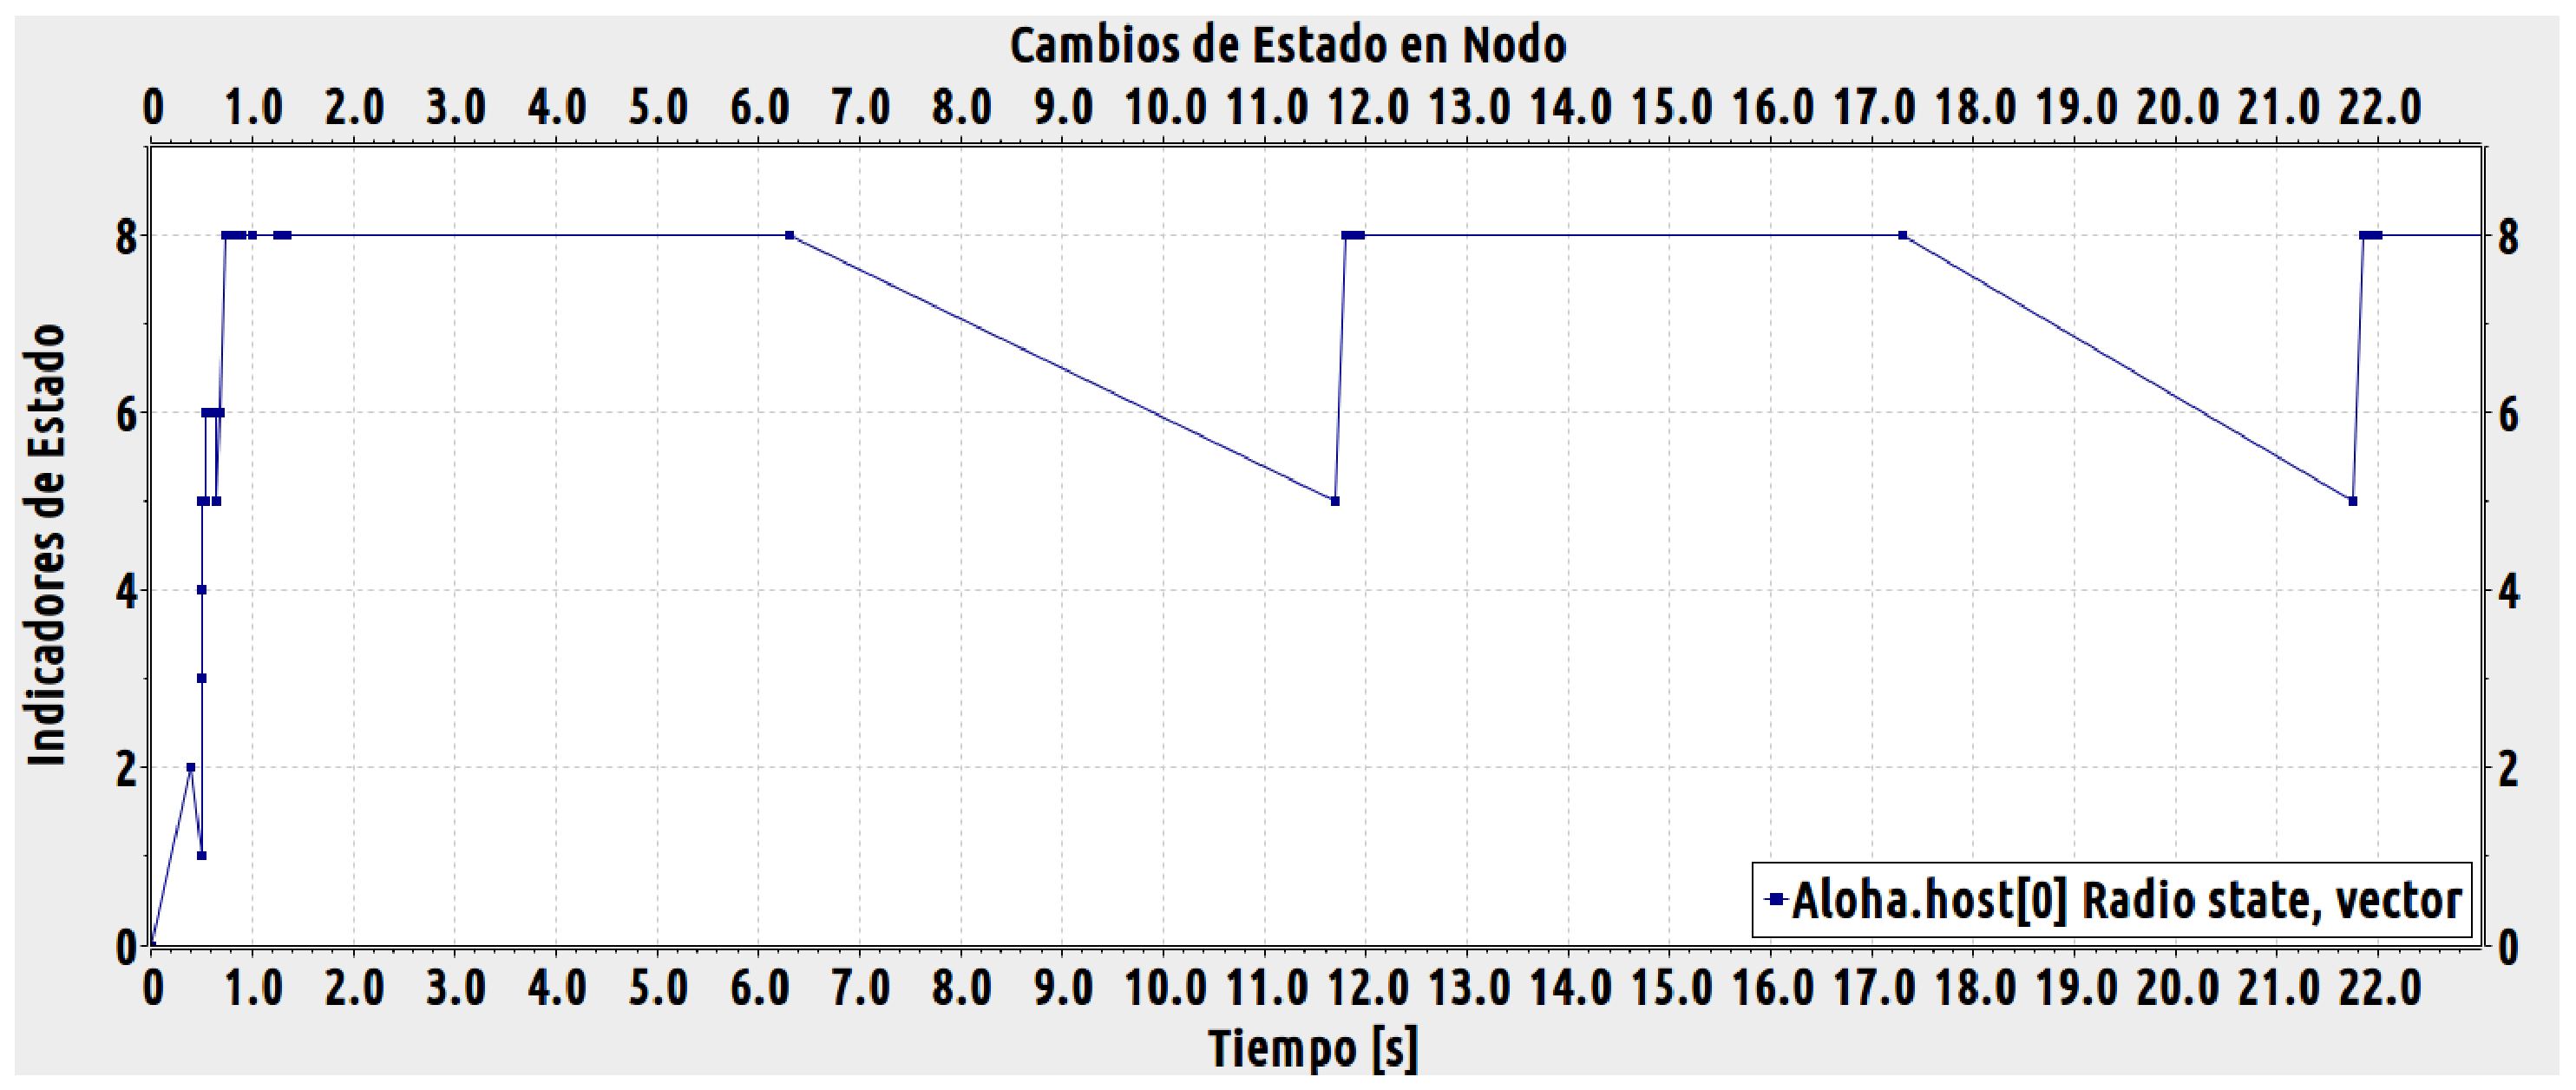
\includegraphics[width=13cm,height=30cm,keepaspectratio]{images/cambioestado1nodo-ideal.eps}
\caption{Gráfico de cambios de estado por tiempo en segundos, con un nodo transmitiendo. \textit{Esta imagen puede verse ampliada en el Anexo~\ref{anexa:1}}}
\label{prueba:1}
\end{figure}
En la Fig~\ref{prueba:2} se encuentra un gráfico de cambios de estado según el tiempo transcurrido, pero esta vez con 10 nodos, con el fin de determinar cuanto demoran los nodos en realizar el proceso de emparejamiento con más nodos por canal.\\
%% pruebas con 10 nodos
\begin{figure}[!ht]
\centering
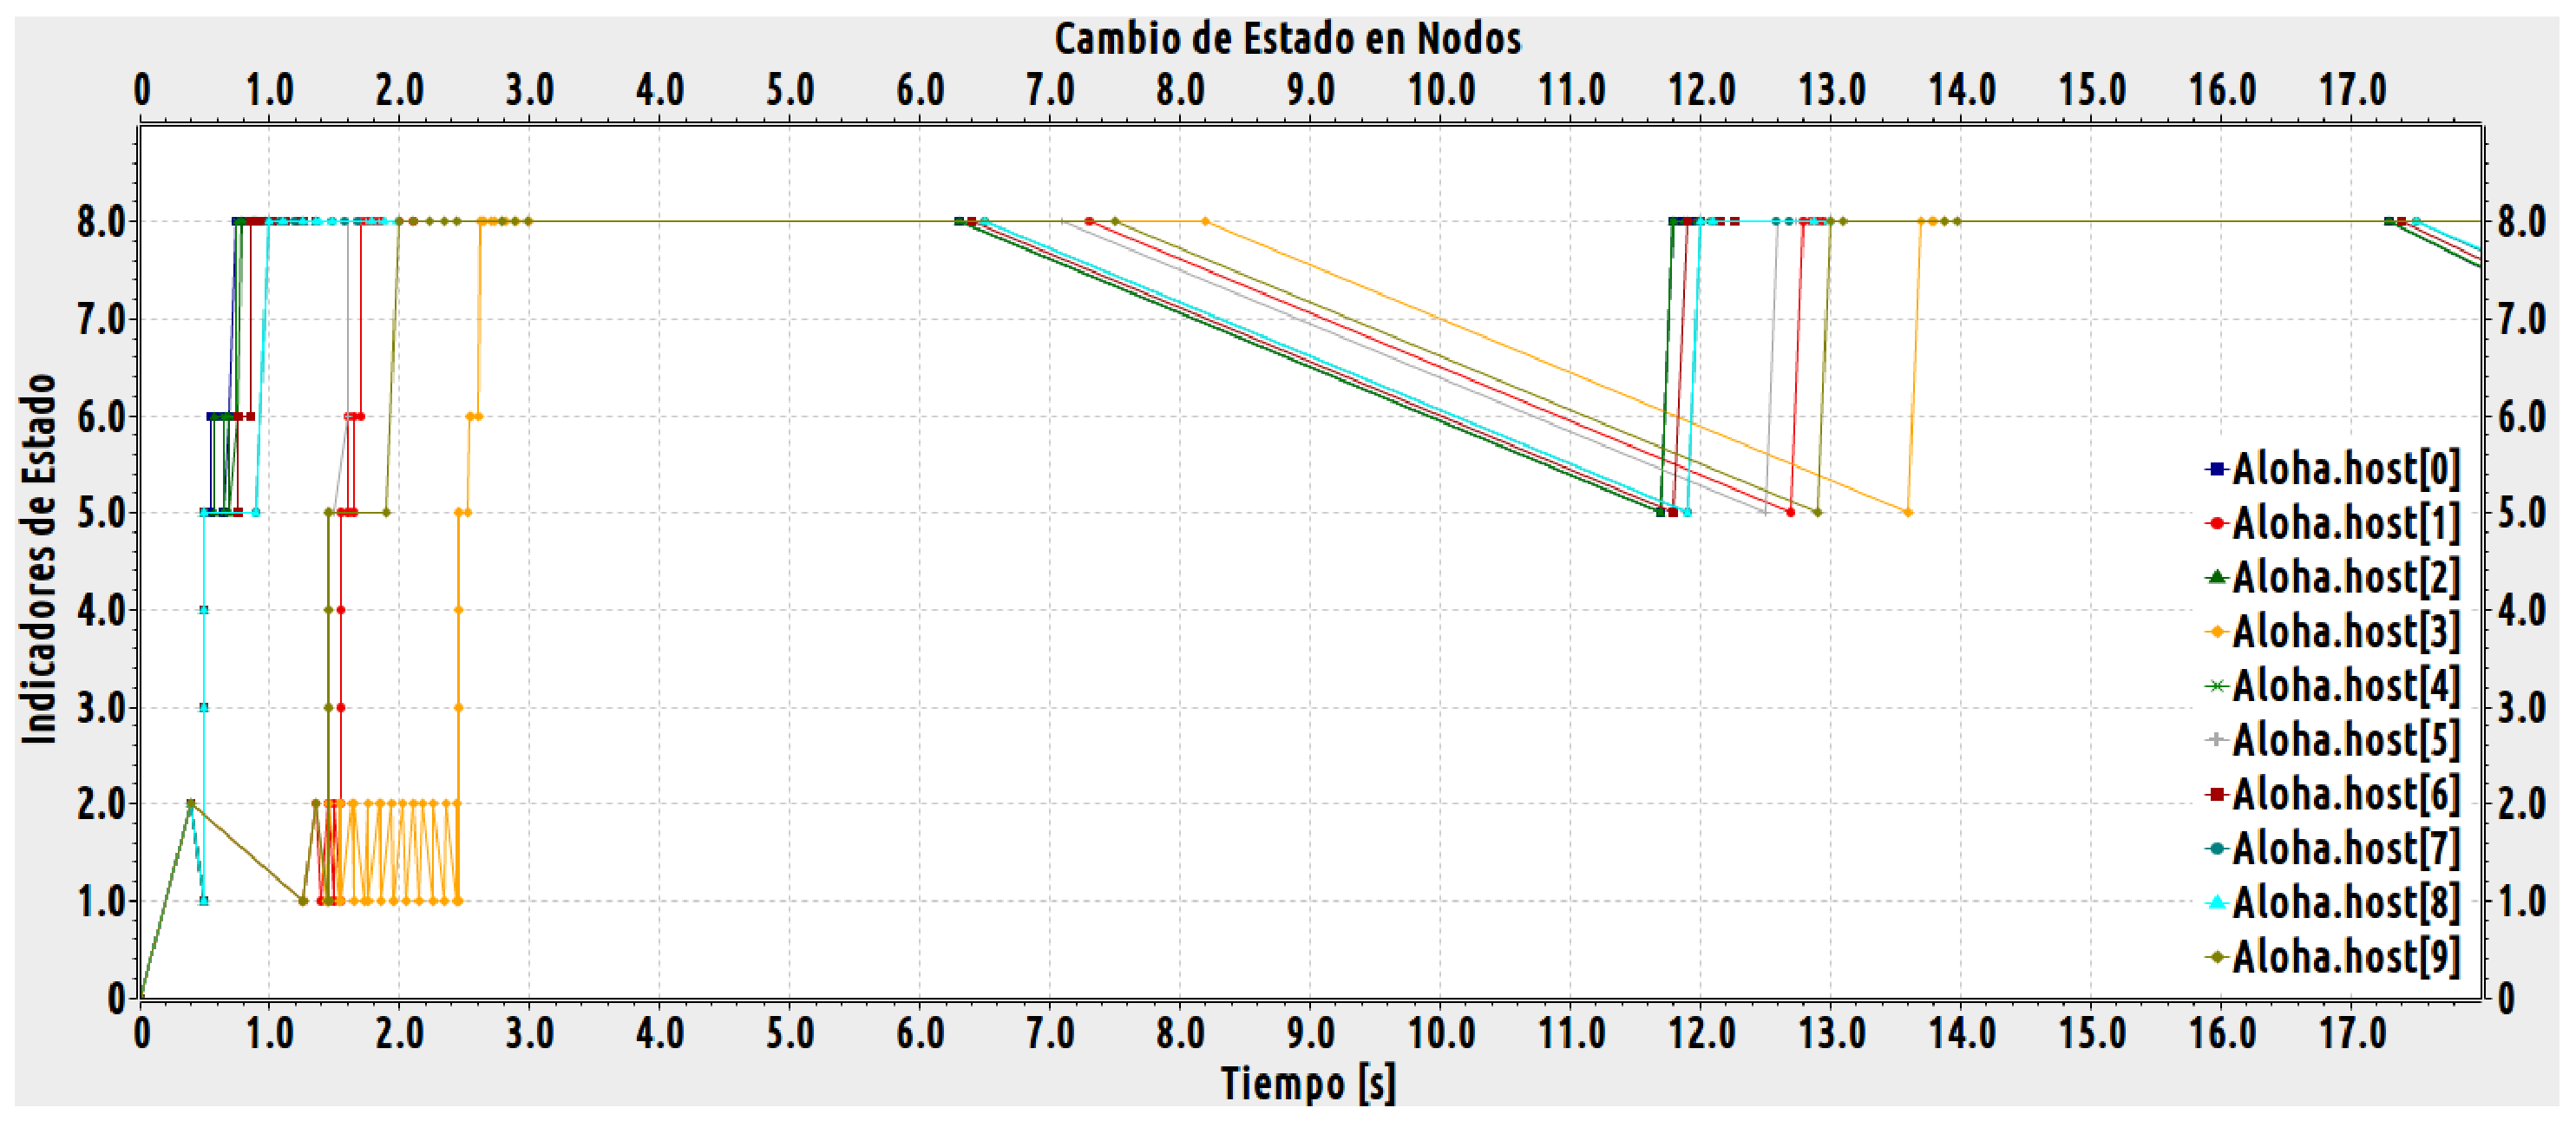
\includegraphics[width=13cm,height=30cm,keepaspectratio]{images/cambioestado10nodos.eps}
\caption{Gráfico de cambios de estado por tiempo en segundos, con diez nodos transmitiendo. \textit{Esta imagen puede verse ampliada en el Anexo~\ref{anexa:2}}}
\label{prueba:2}
\end{figure}
En la Fig~\ref{prueba:3} se presenta un gráfico de cambios de estado donde esta vez se encuentran 100 nodos distribuidos de forma homogénea en los distintos canales disponibles.\newpage \noindent
En estos gráfico, se aprecia de que a medida de que aumenta la cantidad de nodos, el proceso de emparejamiento se ve ralentizado, dado que las colisiones dentro del canal comienzan a generar retransmisiones, las que poco a poco permiten el emparejamiento del total de nodos de la red, y dando inicio al ciclo de transmisión de datos (de medición, u otro tipo) desde los nodos al \textit{gateway}, para luego volver al estado de reposo hasta la próxima ventana de envío.\\
\begin{figure}[!ht]
\centering
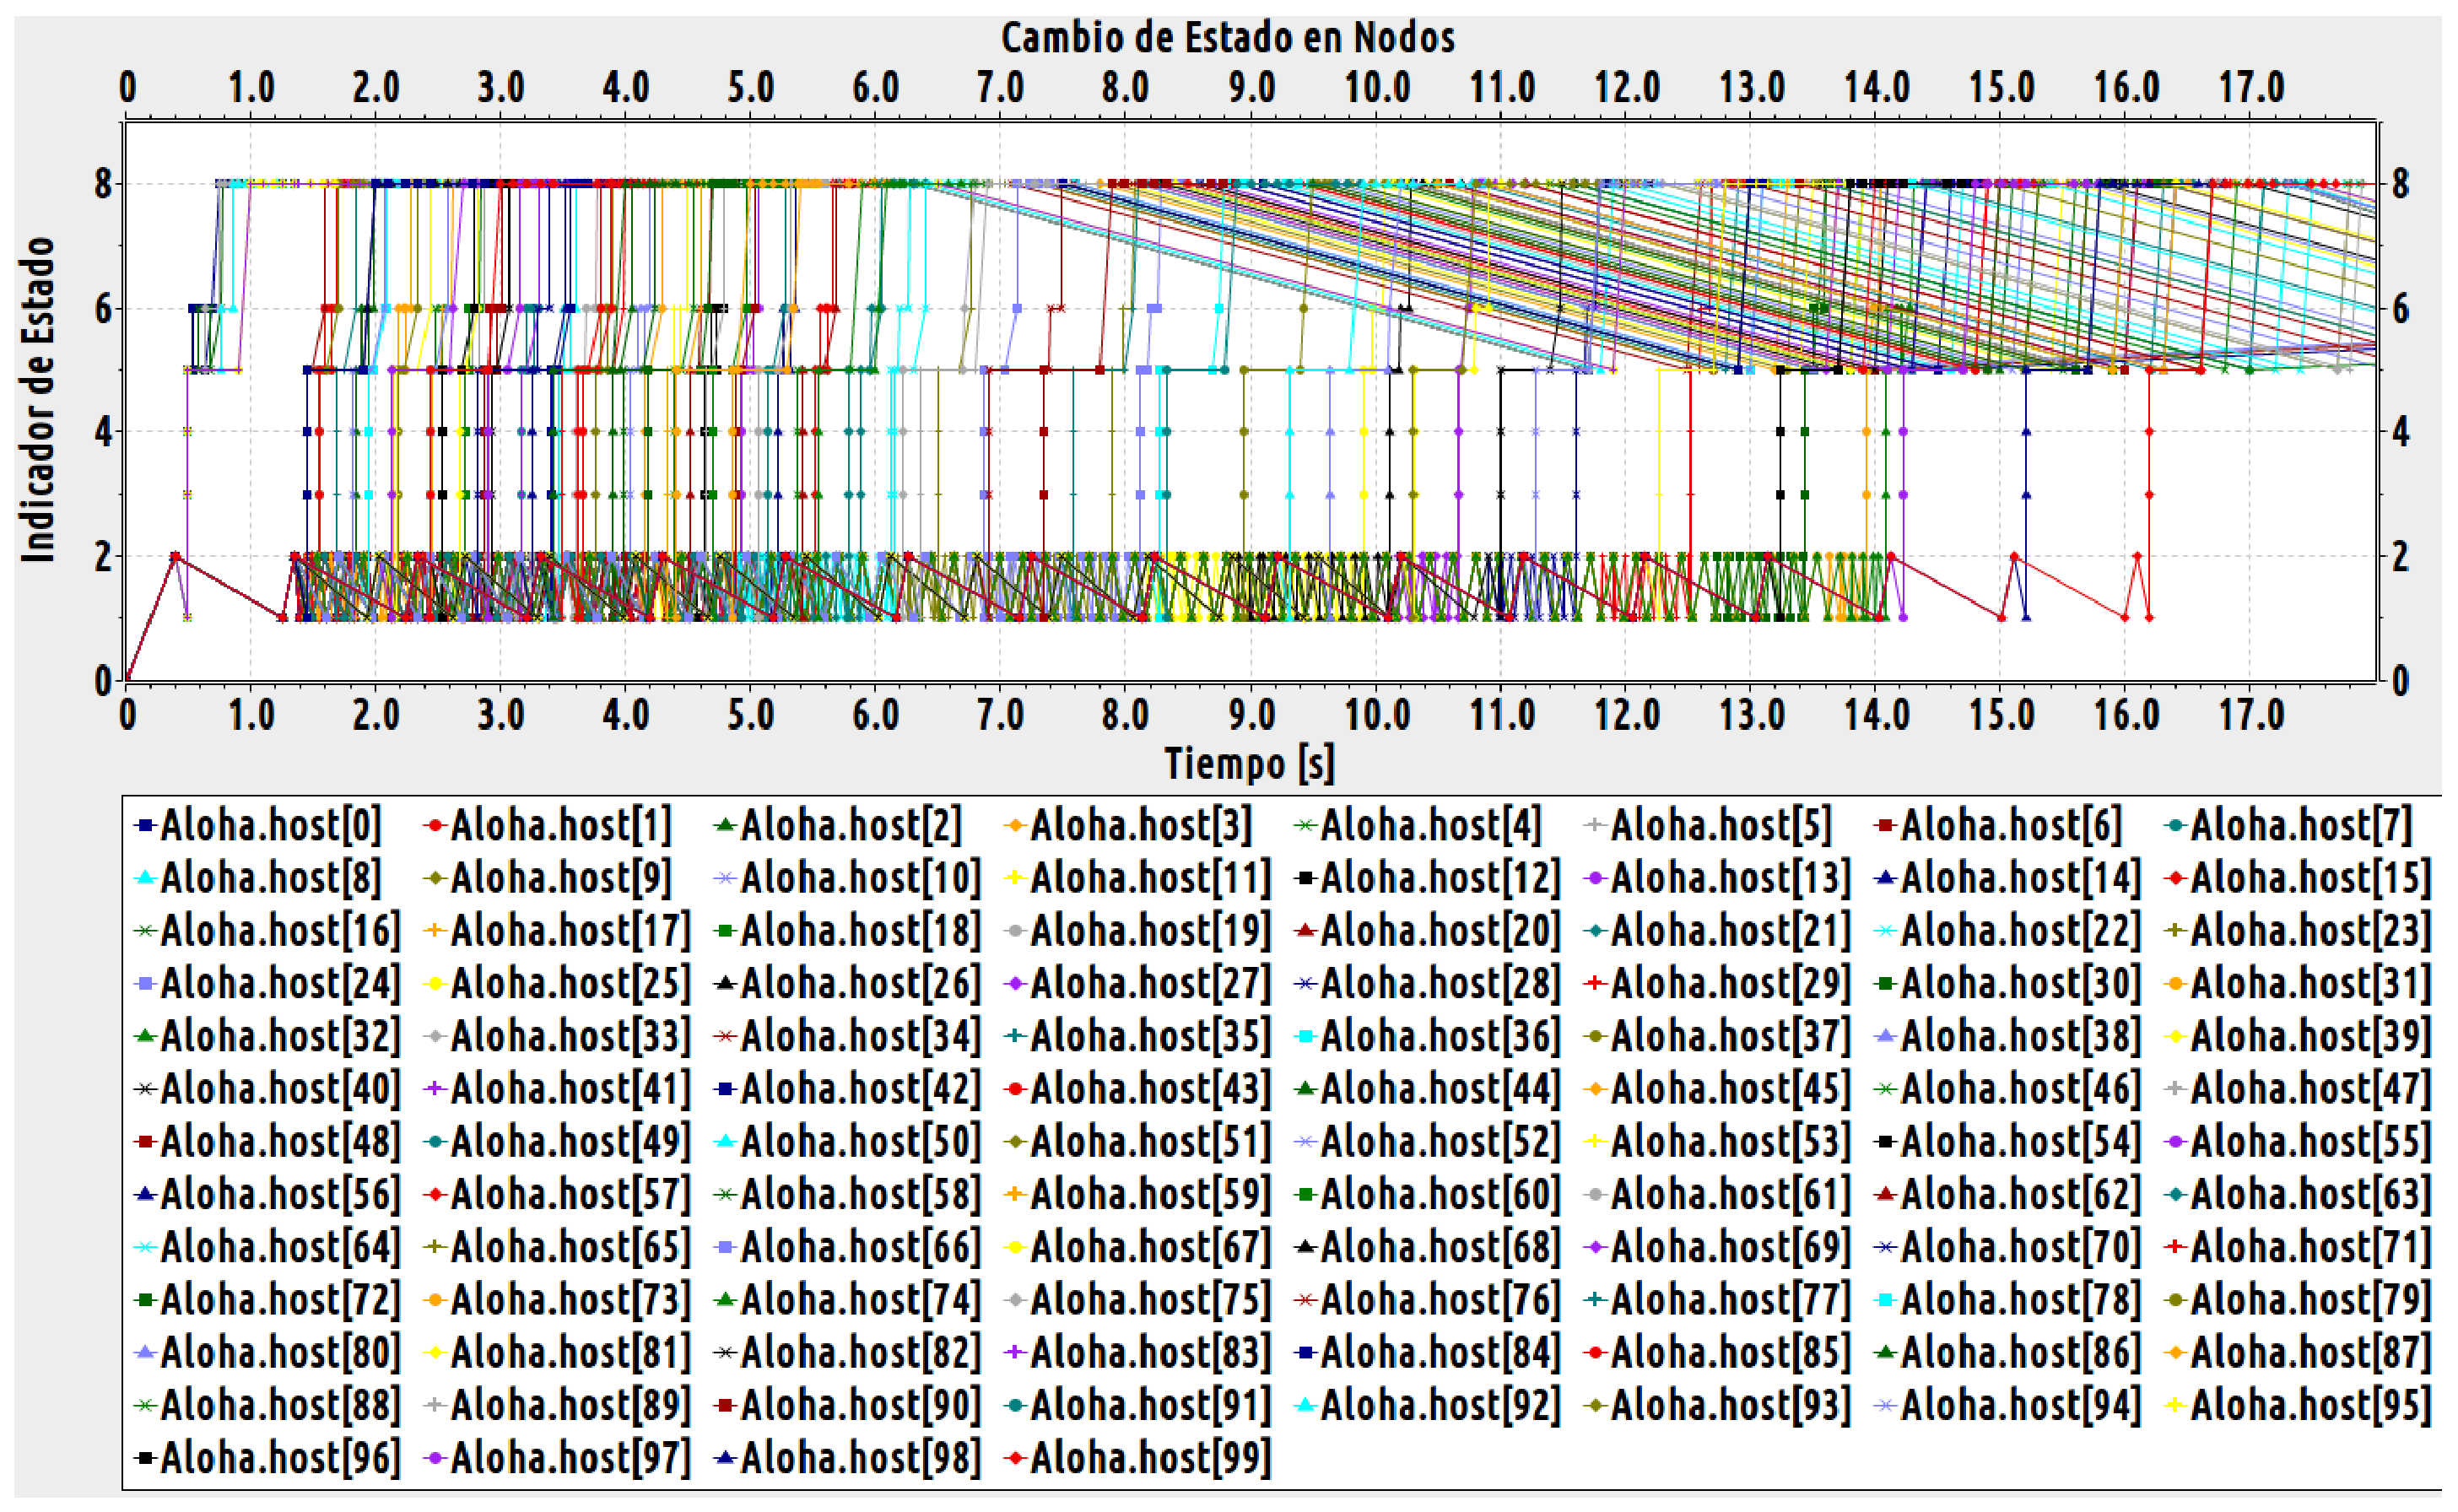
\includegraphics[width=13cm,height=30cm,keepaspectratio]{images/cambioestado100nodos.eps}
\caption{Gráfico de cambios de estado por tiempo en segundos, con cien nodos transmitiendo. \textit{Esta imagen puede verse ampliada en el Anexo~\ref{anexa:3}}}
\label{prueba:3}
\end{figure}
\subsection{Pruebas de transmisión en ambiente virtual}
En estas pruebas, se realizaron transmisiones de datos entre diez y cien nodos durante \SI{60}{\second} de simulación, con el fin de detectar la cantidad de colisiones , por el aumento de la saturación de los canales utilizados. El tiempo de duración de las pruebas de simulación se debe a que en \SI{60}{\second}, es posible visualizar la correcta transición de todos los estados de comunicación presentes en el modelo de simulación, hasta un número de 100 nodos. El valor de la duración de la simulación, fue alcanzado mediante un proceso de optimización de los resultados, donde mediante la realización reiterada de pruebas con resultados no representativos, se alcanzó el tiempo de \SI{60}{\second}. Cabe destacar, que si bien en la simulación transcurre durante \SI{60}{\second}, los gráficos de cambios de estado, sólo muestran dos iteraciones completas del ciclo completo, para evitar mostrar redundancia en los resultados expuestos en los gráficos. No obstante, para el resto de los gráficos, si son utilizados los valores obtenidos durante los \SI{60}{\second} de simulación.\\
Por otra parte, se define el inicio de transmisión de todos los nodos presentes en una simulación, en el mismo segundo. Sin embargo, la herramienta de simulación al mostrar el intercambio de mensajes de forma gráfica, genera una representación gráfica secuencial (sigue el índice asignado a cada nodo y \gls{sf}), es decir, muestra como el intercambio de mensajes se realizará primero en el nodo de índice 0, que en el nodo 1 (a modo de ejemplo), no obstante, esto no se condice con los tiempos de envío de mensajes en la simulación, dado que ambos intentan comunicarse en el mismo segundo, lo que produce que colisionen mensajes y sean reprogramados para la siguiente ventana de envío. En este punto el simulador genera una distribución nuevamente secuencial, sobre cuál nodo calendariza primero su retransmisión, lo que genera un orden secuencial en el envío de mensajes, pero a nivel de programación. Este factor, afecta a los resultados de la simulación de manera negativa, al alejarlos de la realidad, pero se corrigieron al agregar tiempos aleatorios a la calendarización de las próximas programaciones de envío. Lo que se estudió en base a la diferencia de tiempos de envío entre los nodos una vez secuenciados, con el fin de equiparar el ambiente real con el virtual.\\
A través de estas mediciones, se espera visualizar el creciente nivel de retardo en el inicio de las distintas fases de los nodos por efecto de las colisiones, y las retransmisiones inherentes de comunicaciones basadas en el protocolo ALOHA. Cabe decir de que sólo existen colisiones dentro de cada \gls{sf} o canal, ya que entre los distintos \gls{sf} según las especificaciones técnicas  y según las pruebas empíricas realizadas a las capacidades del canal , se indica de que al usar la técnica de modulación de espectro expandido, basta con conocer la frecuencia base del mensaje para poder recibirlo y demodularlo sin problemas, dado que cualquier interferencia en el resto del espectro de la señal, será eliminado al momento de filtrar la señal con un filtro pasa banda, pasa bajo, entre otros, dependiendo del necesario para cada canal~\cite{Sornin}~\cite{Xavier}.\\
En la Fig~\ref{nodos:10}, se observa la cantidad de colisiones por cada \gls{sf}, donde la utilización de cada canal fue aproximadamente de 2 nodos por canal, lo que eventualmente es una saturación muy baja, lo que se traduce en un retardo pequeño en tiempo de el correcto inicio y finalización de los estados correspondientes a cada fase de la comunicación en los dispositivos LoRa.

\begin{figure}[!ht]
\centering
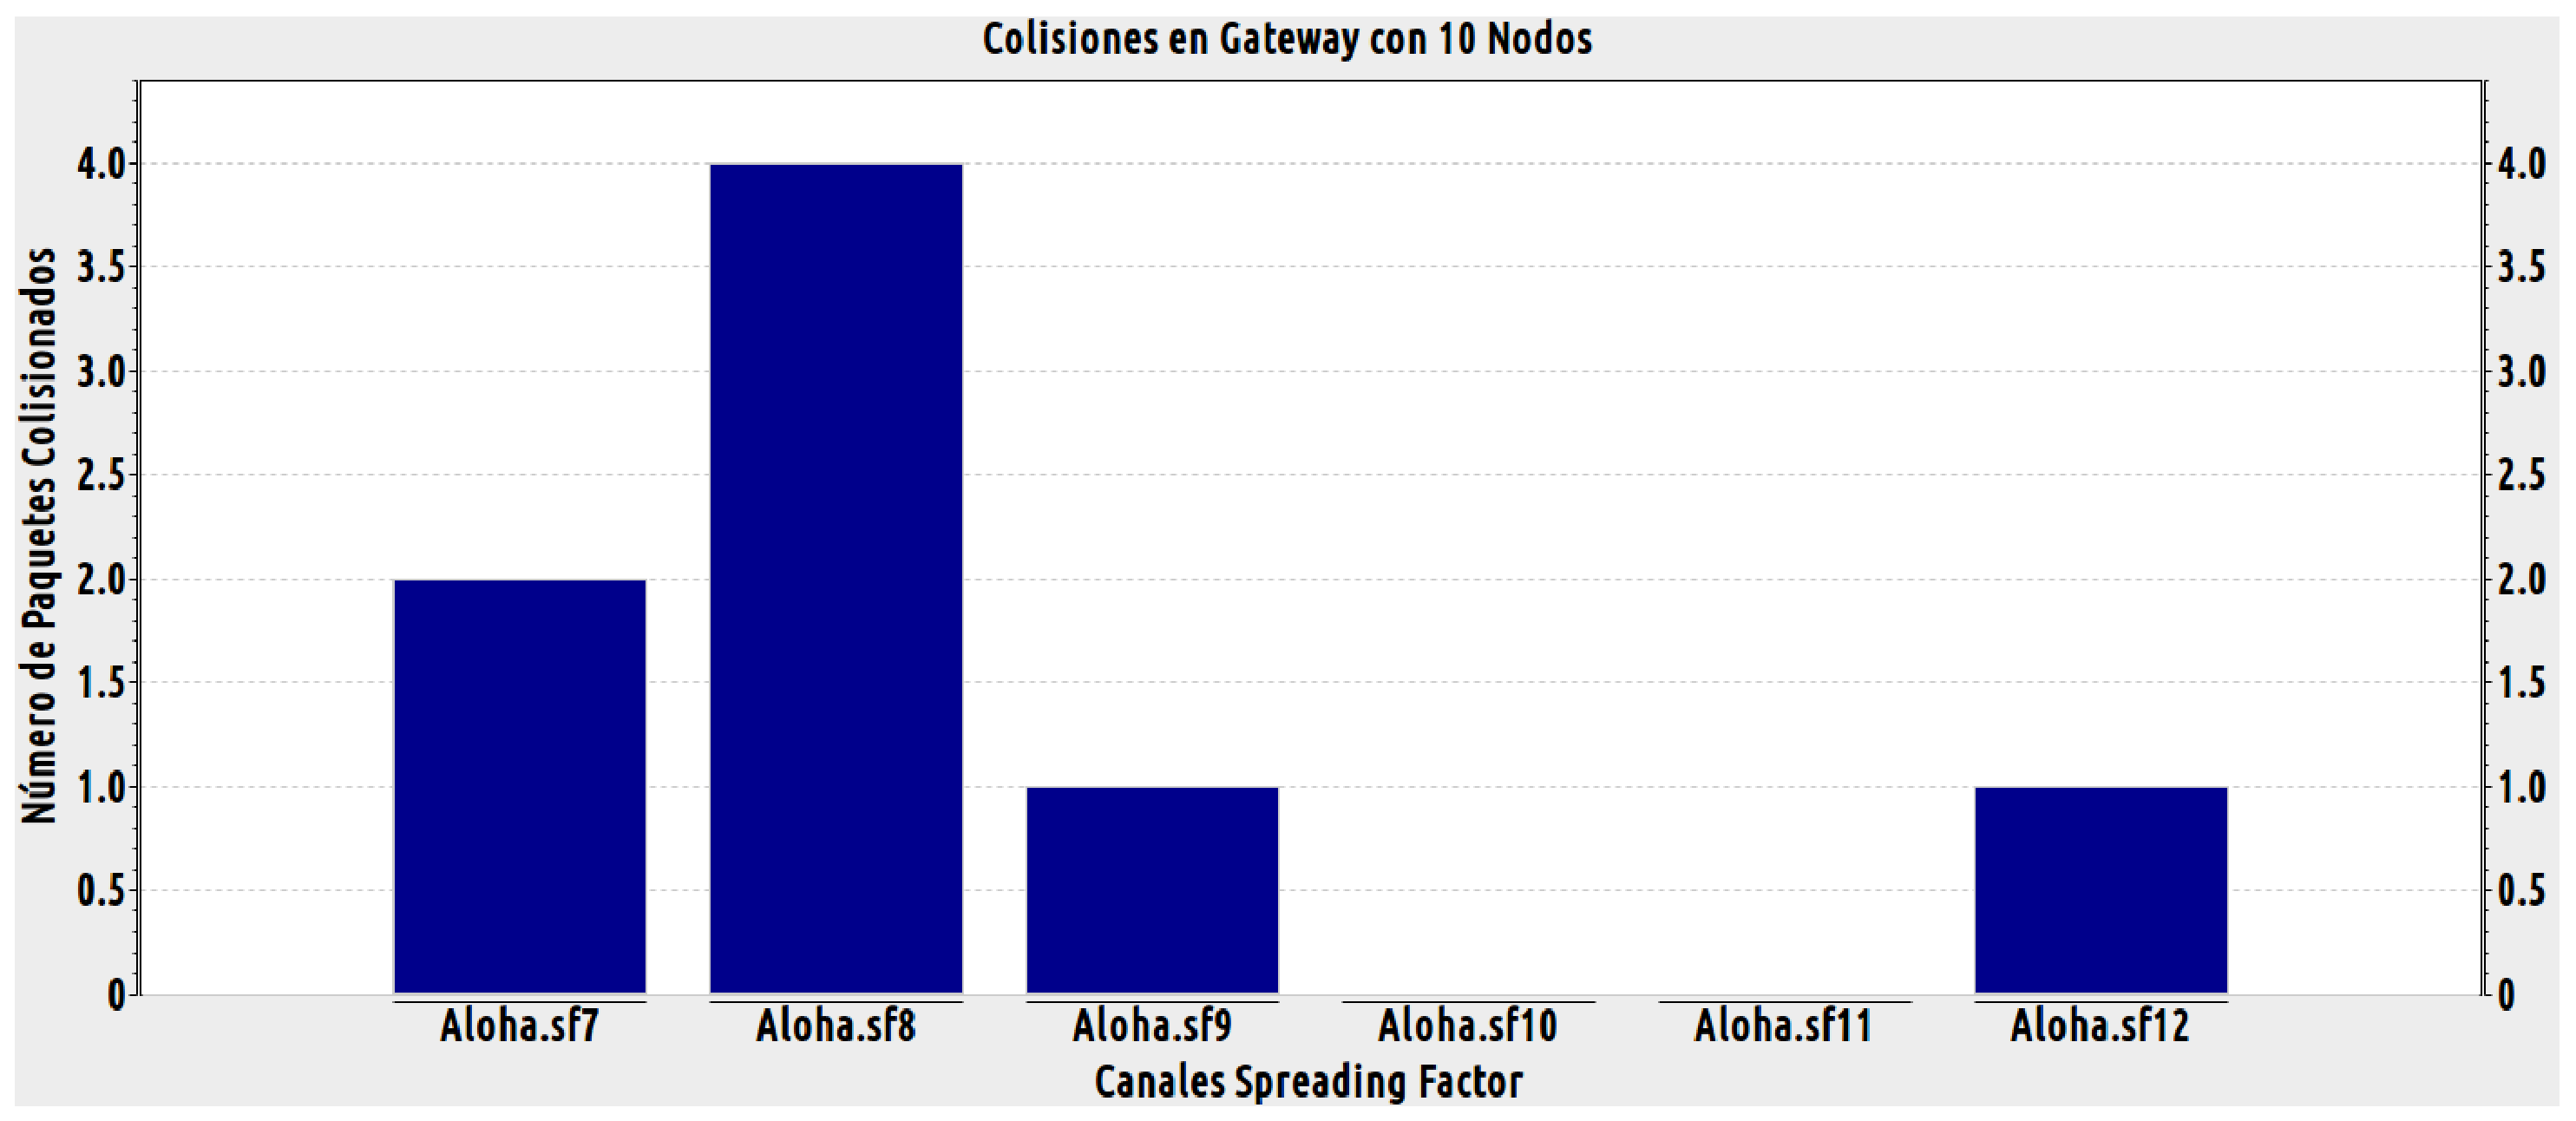
\includegraphics[width=13cm,height=30cm,keepaspectratio]{images/colisiones10nodos.eps}
\caption{Gráfico de colisiones ocurridos entre los distintos \glsentryname{sf}, para 10 nodos transmitiendo. \textit{Esta imagen puede verse ampliada en el Anexo~\ref{anexb:1}}}
\label{nodos:10}
\end{figure}

En la Fig~\ref{nodos:100}, se contempla de que se sigue la misma distribución de colisiones, con la diferencia de que al aumentar los nodos, la saturación del canal  aumenta más de diez veces a la prueba anterior, donde si bien la distribución por canal del número de colisiones se mantiene, la cantidad misma de colisiones no sigue un patrón, lo que puede deberse a un exceso de retransmisiones en el canal produciendo saturación en algún \gls{sf} específico, generando este crecimiento abrupto del número de colisiones. En relación al número de colisiones, estas aumentan también más de diez veces, excepto en el \gls{sf} 8, donde ocurre una anomalía en el comportamiento del modelo de simulación. El cual es explicado por el orden pseudo-aleatorio que posee el \textit{framework} a la hora de indicar que nodo es el siguiente en enviar datos, esto conlleva a que sólo este \gls{sf}, posea este comportamiento fuera de lo normal (como el resto de los \gls{sf}). Adicionalmente, los \gls{sf} 10 y 11, también presentan un crecimiento fuera del patrón (considerando que no habían colisiones con 10 o menos nodos), pero esto tiene relación con el número de nodos por canal, donde la distribución de nodos expuesta en Tab~\ref{tab:prueba} indica de que los canales con sólo un nodo son justamente el \gls{sf} 10 y 11. Esta distribución de nodos por \gls{sf}, se define para probar tanto canales con distribución uniforme, como también la interacción en simultaneo con canales con menor utilización de canal, con el fin de evaluar diferencias de utilización de canal y nivel de colisiones, que es lo que se presenta en este apartado.\\
La diferencia de valores entre \gls{sf} también es explicada por el hecho de que la simulación fue tomada en sólo \SI{60}{s} de simulación, a modo de optimizar los resultados de la medición, dado que en este tiempo, fue posible medir para todos los casos propuestos, el transcurso de todas las fases de comunicación en todos los nodos. Por esta razón, lo que los gráficos muestran, es el estado de la simulación en ese momento dado. Sin embargo, en el caso de haber permitido seguir la simulación una cantidad de segundos más, se apreciaría un emparejamiento del número de colisiones obtenidas en todos los \gls{sf}. Si bien, se realiza esta observación, dado que el \gls{per} agregado al modelo de simulación, recalcula su valor para cada \gls{sf}, cada vez que se recibe un mensaje en cada \gls{sf}. Esto genera, que no se pueda obtener el valor óptimo para esta medición, dado que siempre está recalculando por lo que se entra en un búcle. Por esta razón se estableció un tiempo para tomar la medición de este error, donde en base a prueba y error, se estableció de que a los \SI{60}{s} es posible obtener los mejores resultados para esta prueba (valores más parejos entre los \gls{sf}). Este índice depende mucho de en que fase se encuentren en ese segundo y que evento está queriendo representar. Para este caso en particular, no es importante el hecho de esta anormalidad, dado que se logra explicar el porqué del evento, junto con poder analizar el crecimiento del número de colisiones a mayor número de nodos.
\begin{figure}[!ht]
\centering
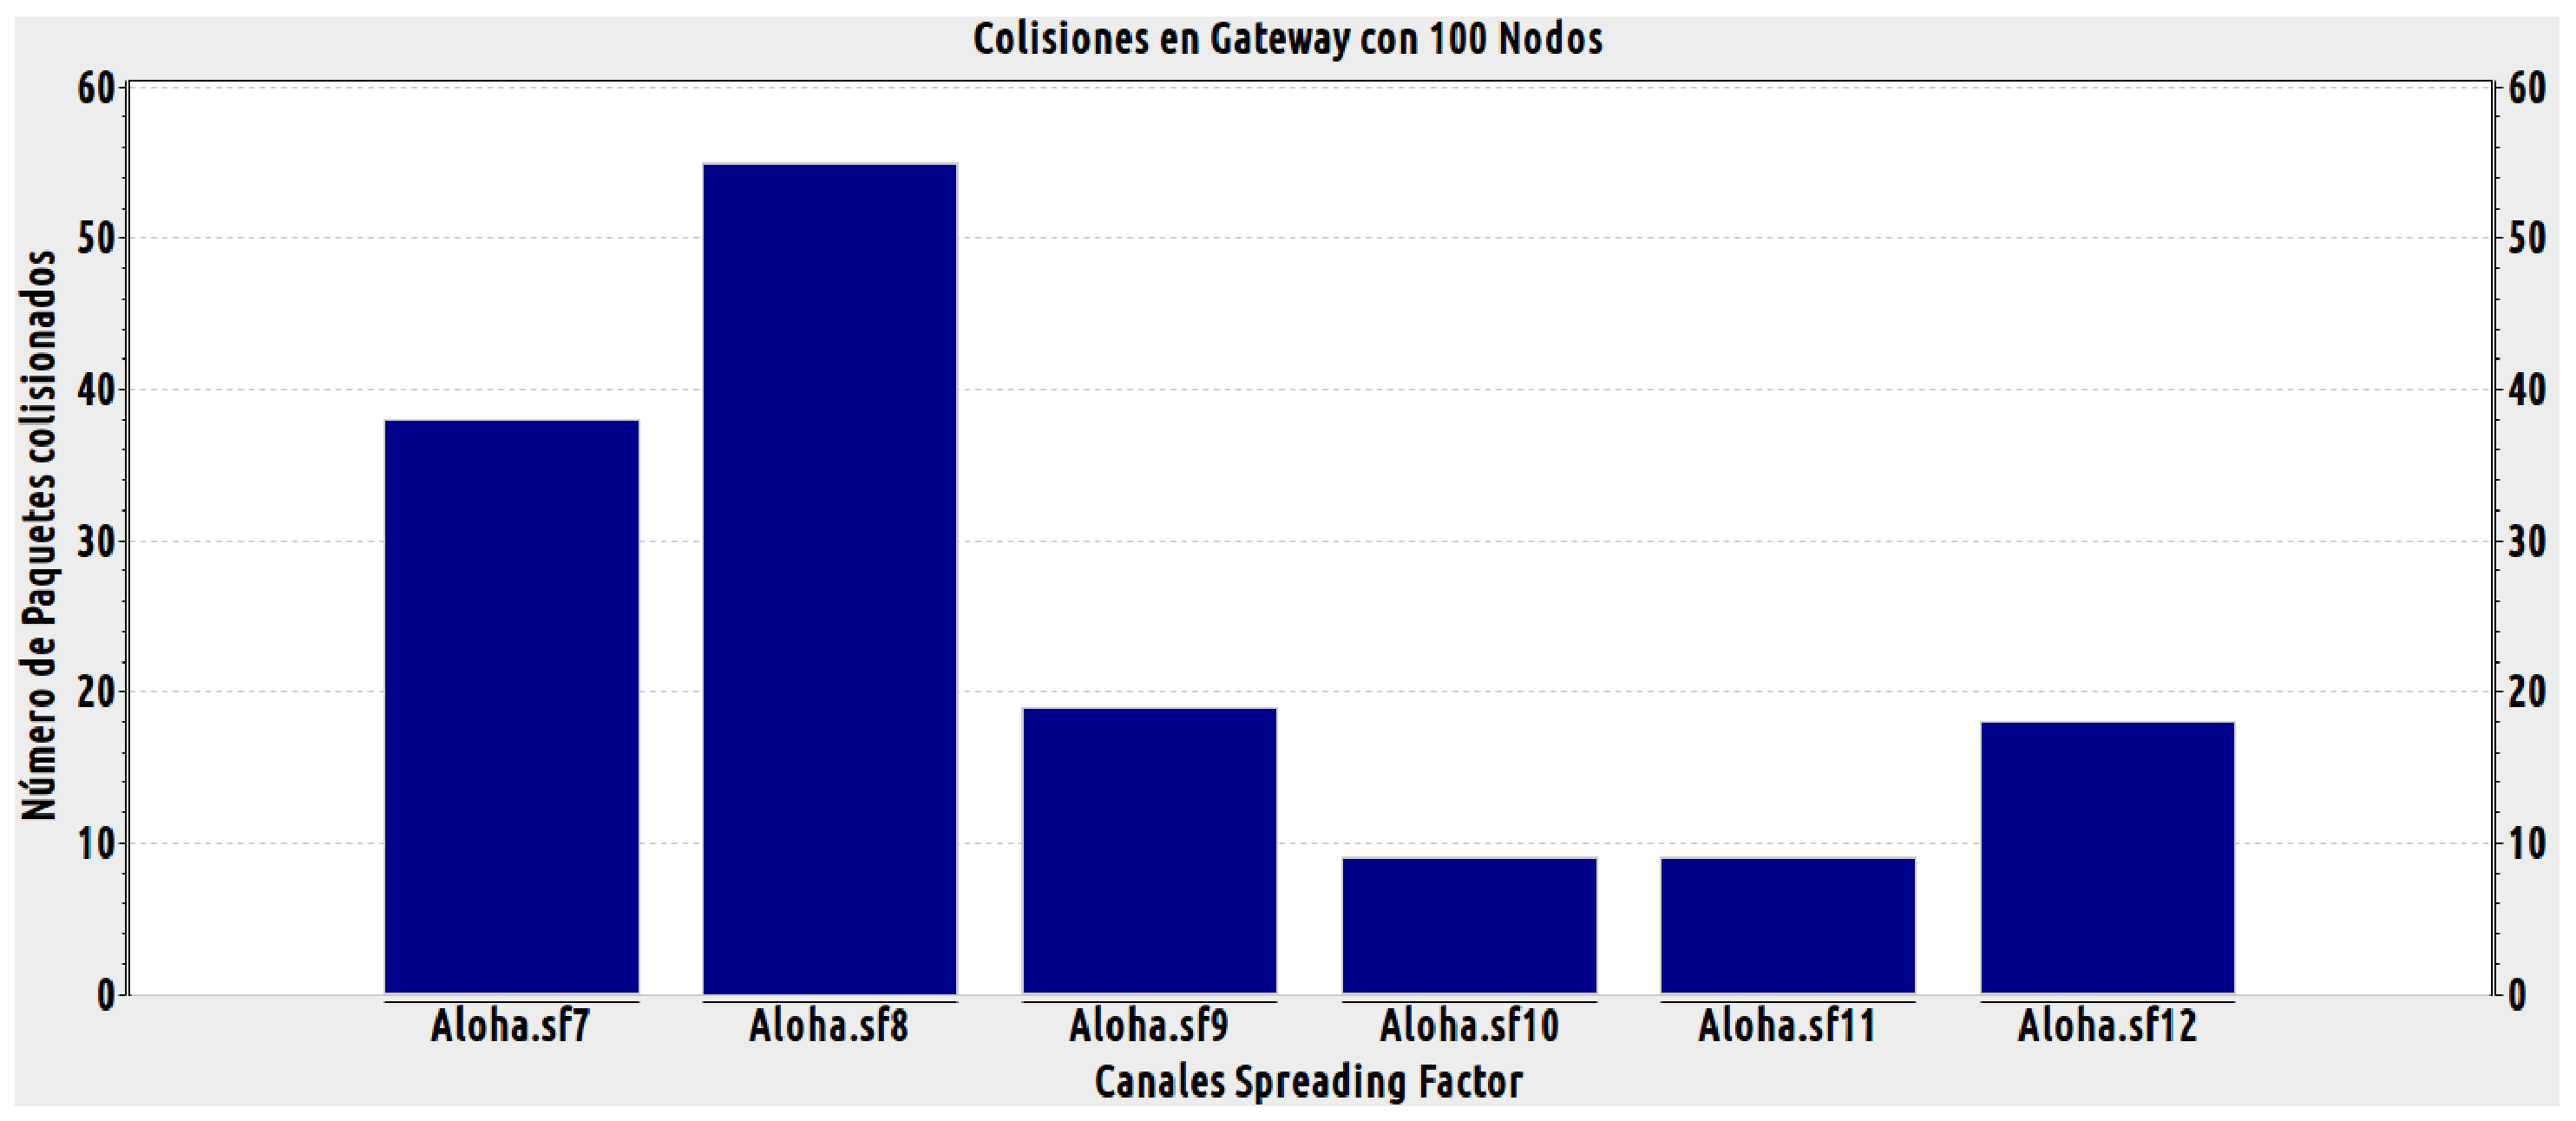
\includegraphics[width=13cm,height=30cm,keepaspectratio]{images/colisiones100nodos.eps}
\caption{Gráfico de colisiones ocurridos entre los distintos \glsentryname{sf}, para 100 nodos transmitiendo. \textit{Esta imagen puede verse ampliada en el Anexo~\ref{anexb:2}}}
\label{nodos:100}
\end{figure}
\subsection{Pruebas de transmisión en ambiente real}
Para realizar las pruebas de transmisión en ambientes reales con los dispositivos LoRa, se utilizó como \textit{gateway} un concentrador LoRa c880A con una antena omnidireccional que trabaja en la banda de frecuencia \SI{868}{\mega\hertz}, que posee \SI{5}{dbi} de sensibilidad, adicionalmente se transmitió con una potencia de \SI{10}{dbm}. Este dispositivo fue conectado a una Raspberry Pi 2. Como nodo se utilizó un inAir9 (LoRa Module \SI{868}{\mega\hertz}), el que tuvo conectada una antena omnidireccional con una sensibilidad de \SI{5}{dbi} y tuvo configurada una potencia de transmisión de \SI{10}{dbm}. El nodo se conectó a un arduino UNO el que funcionó como \textit{backend}. La distancia entre el nodo y el \textit{gateway} fue de \SI{20}{\meter} aproximadamente sin obstaculos entre ellos. En relación a la altura del \textit{gateway}, esta fue de \SI{1.2}{\meter} aproximadamente, la que se debe a la altura de una mesa, ubicada en las áreas verdes de la facultad de ingeniería de la Universidad Diego Portales. Por otro lado la del nodo fue de \SI{0.9}{\meter} aproximadamente, altura debida al bloque de cemento utilizado como base del nodo.\\
Las pruebas de transmisión, se realizaron cinco veces para cada \gls{sf}, con el fin de determinar el porcentaje de pérdida de paquetes en cada espectro de frecuencia y agregarlo al modelo de simulación. \noindent
La cantidad de iteraciones del experimento de transmisión, se debe a un proceso de optimización en los resultados del experimento, es decir, a medida que se realizaron las mediciones, se procedió a ajustar el número de iteraciones sobre la base de los resultados obtenidos. Como puede apreciarse en Tab~\ref{prueba:real}, en esta prueba se enviaron en promedio noventa y siete paquetes de datos, de los cuales sólo se recibió alrededor de treinta y siete en promedio, lo que corresponde a un \SI{38}{\percent} de recepción de los datos enviados en el total de paquetes enviados. Sin embargo, algunos resultados en las mediciones tuvieron una diferencia considerable de resultados (véase [*] en Tab~\ref{prueba:real}), valores que son explicados si se toma en cuenta que los valores expuestos en la tabla de resultados son promedios de todas las pruebas realizadas por cada canal de comunicaciones, donde cabe destacar, que las intensidades de las interferencias a las que estaban sometidos los dispositivos al momento de las mediciones eran variables, lo que explica el por qué el valor en el \gls{sf}9 posee una desviación alta en comparación con los valores de los otros canales. Los valores que provocan esta desviación en el \gls{sf}9, no fueron quitados con el fin de mostrar de que en algunos casos se lograron valores de recepción altos en las mediciones, con respecto a la pérdida de paquetes (valores bajo el \SI{10}{\percent} en \gls{per}), como también valores bajos en relación a la recepción de paquetes (valores de \gls{per} sobre el \SI{70}{\percent}). Estos resultados en la mayoría de los casos, mostraron una tendencia a obtener valores de \gls{per} altos, excepto en el canal \gls{sf}9, donde hubo una mayor incidencia de recepción exitosa de mensajes que en el resto de canales.\\
La configuración de parámetros usada para esta prueba, junto con la arquitectura de red usada corresponden a los valores y distribuciones definidos en la sección~\ref{sec:param}. A continuación se presentan los resultados:
\begin{table}[!ht]
\centering
\begin{tabular}{|c|c|c|c|}
\hline
\gls{sf} & Paquetes enviados & Paquetes recibidos & Paquetes perdidos \SI{}{\percent} \\ 
\hline
SF12 & 84 & 30 & \SI{65,1}{\percent}\\
\hline
SF11 & 99 & 15 & \SI{84,8}{\percent}\\
\hline
SF10 & 158 & 19 & \SI{87.9}{\percent}\\
\hline
SF9 & 360 & 78 & \SI{78.3}{\percent}[*]\\
\hline
SF8 & 469 & 38 & \SI{91.9}{\percent}\\
\hline
SF7 & 983 & 47 & \SI{95.2}{\percent}\\
\hline
\end{tabular}
\caption{Tabla con resultados de pruebas de conectividad por \glsentryname{sf}}
\label{prueba:real}
\end{table}
\newpage \noindent
Bajo este contexto, estos resultados sirvieron para el modelado de los dispositivos LoRa, dado que en un principio se definió que se dejaría un valor fijo de pérdida de paquetes para representar el estándar expuesto en las especificaciones de los desarrolladores de LoRa, sin embargo, estos resultados revelaron de que la variabilidad de resultados respecto a la recepción de datos, depende de tres factores principales: la potencia de transmisión, la sensibilidad de recepción y el uso del espectro expandido. En relación a estos antecedentes, se estableció de que se modelaría de forma dinámica la pérdida de paquetes, con el fin de adaptar el modelo de simulación a cualquier tipo de ambiente a simular, sin que este pierda similitud con el comportamiento real en los dispositivos.
\subsection{Índice de pérdida de paquetes}
En relación a las pruebas de transmisión realizadas con los dispositivos físicos, se alejan mucho de los resultados esperados, e incluso de los datos que otorga la especificación de LoRa. Esto es causado por la interferencia generada por la fuente de poder administrada a los dispositivos y una incorrecta forma de aislamiento de los conectores y partes conductoras de la placa. Adicionalmente, se considera de que que sea producto de la baja potencia de transmisión del \textit{gateway} (\SI{5}{dbm}), e incluso de la alta sensibilidad de la antena de transmisión (\SI{5}{dbi}) dado que esto la hace más permeable a interferencias ambientales propias de una universidad. Adicionalmente, se considera la baja altura a la que se colocó el \textit{gateway} (\SI{1.2}{\meter}), como un factor negativo en las mediciones, dado que los dispositivos estuvieron a baja altura, estos pudieron ser afectados por radiación de electrodomésticos. Por otra parte, todas las pruebas realizadas por investigadores, tanto las pruebas realizadas a la capacidad del canal, como a la capacidad de transmisión, los resultados arrojan que sus pruebas son muy satisfactorias dado que sus resultados, se apegan a las especificaciones técnicas entregadas por Semtech en condiciones dentro de las normas expuestas allí.\noindent 
Dentro de las características de estas pruebas, se encuentra que los \textit{gateway} están ubicados a una altura de sobre los \SI{20}{\meter} en torres fijas, y equipados con antenas bi-cónicas con una sensibilidad de \SI{2}{dbi}, y transmitiendo a una potencia de (\SI{14}{dbm}), lo que permite una transmisión a mucha más distancia que el mismo \textit{gateway} a una menor altura, donde la calidad de transmisión puede verse mermada por las interferencias a ese nivel de altura, agregando a este análisis, de que las antenas utilizadas en los experimentos expuestos en los artículos citados, están diseñadas para la comunicación direccional en sus dos polos, lo que aumenta el nivel de emisión y recepción en estas direcciones, a diferencia de la omni direccional que se utilizó para estas mediciones, que posee un mayor nivel de pérdida en ciertos polos~\cite{Xavier}~\cite{Juha}~\cite{NORMAN}.\\
De acuerdo a este contexto, se decidió adoptar el porcentaje de pérdida de paquetes que entregan las distintas mediciones realizadas por otros investigadores (tasa de pérdida de paquetes = \SI{1}{\percent}), se asemejan más a la norma y a las especificaciones~\cite{Xavier}~\cite{Juha}.

\subsection{Resultados obtenidos agregando pérdida de paquetes}
Dentro de las pruebas de transmisión en el ambiente virtual, también se registró la cantidad de paquetes con errores (que no llegaron a destino), los que en un ambiente real pueden tener el carácter de interferencia. Para el modelo de simulación el porcentaje de pérdida en la recepción de datos, se mide en cada transmisión en base al \gls{per} ingresado, junto a la cantidad de paquetes recibidos por cada \gls{sf}, por lo que dependiendo de que \gls{sf} posea más envíos efectivos de mensajes (en el caso de que uno haya entrado antes al estado de transmisión que otro nodo).\\
Como es posible notar en la Fig~\ref{prueba:4}, la cantidad de envíos de datos con errores es igual en los \gls{sf}7, 8 y 12 (con un \gls{per} del \SI{1}{\percent}), excepto en los \gls{sf}9 \gls{sf}10 y \gls{sf}11 donde se presenta un valor menor. Ésto es debido a que los \gls{sf} afectados, transmitieron entre 10-50 paquetes menos que el resto de los \gls{sf}. Cabe mencionar de que, en el caso de que la simulación hubiera continuado, es posible de que el índice \gls{per} se hubiera vuelto homogéneo en todos los \gls{sf}.\\
Estos resultados al ser satisfactorios, demuestran de que con diez nodos, la función que calcula esta pérdida es efectiva dependiendo del número de paquetes recibidos, por lo que se concluye que es efectiva en un nivel bajo de saturación de canal (bajo 50 nodos por canal).
%%pruebas con 5 nodos
\begin{figure}[!ht]
\centering
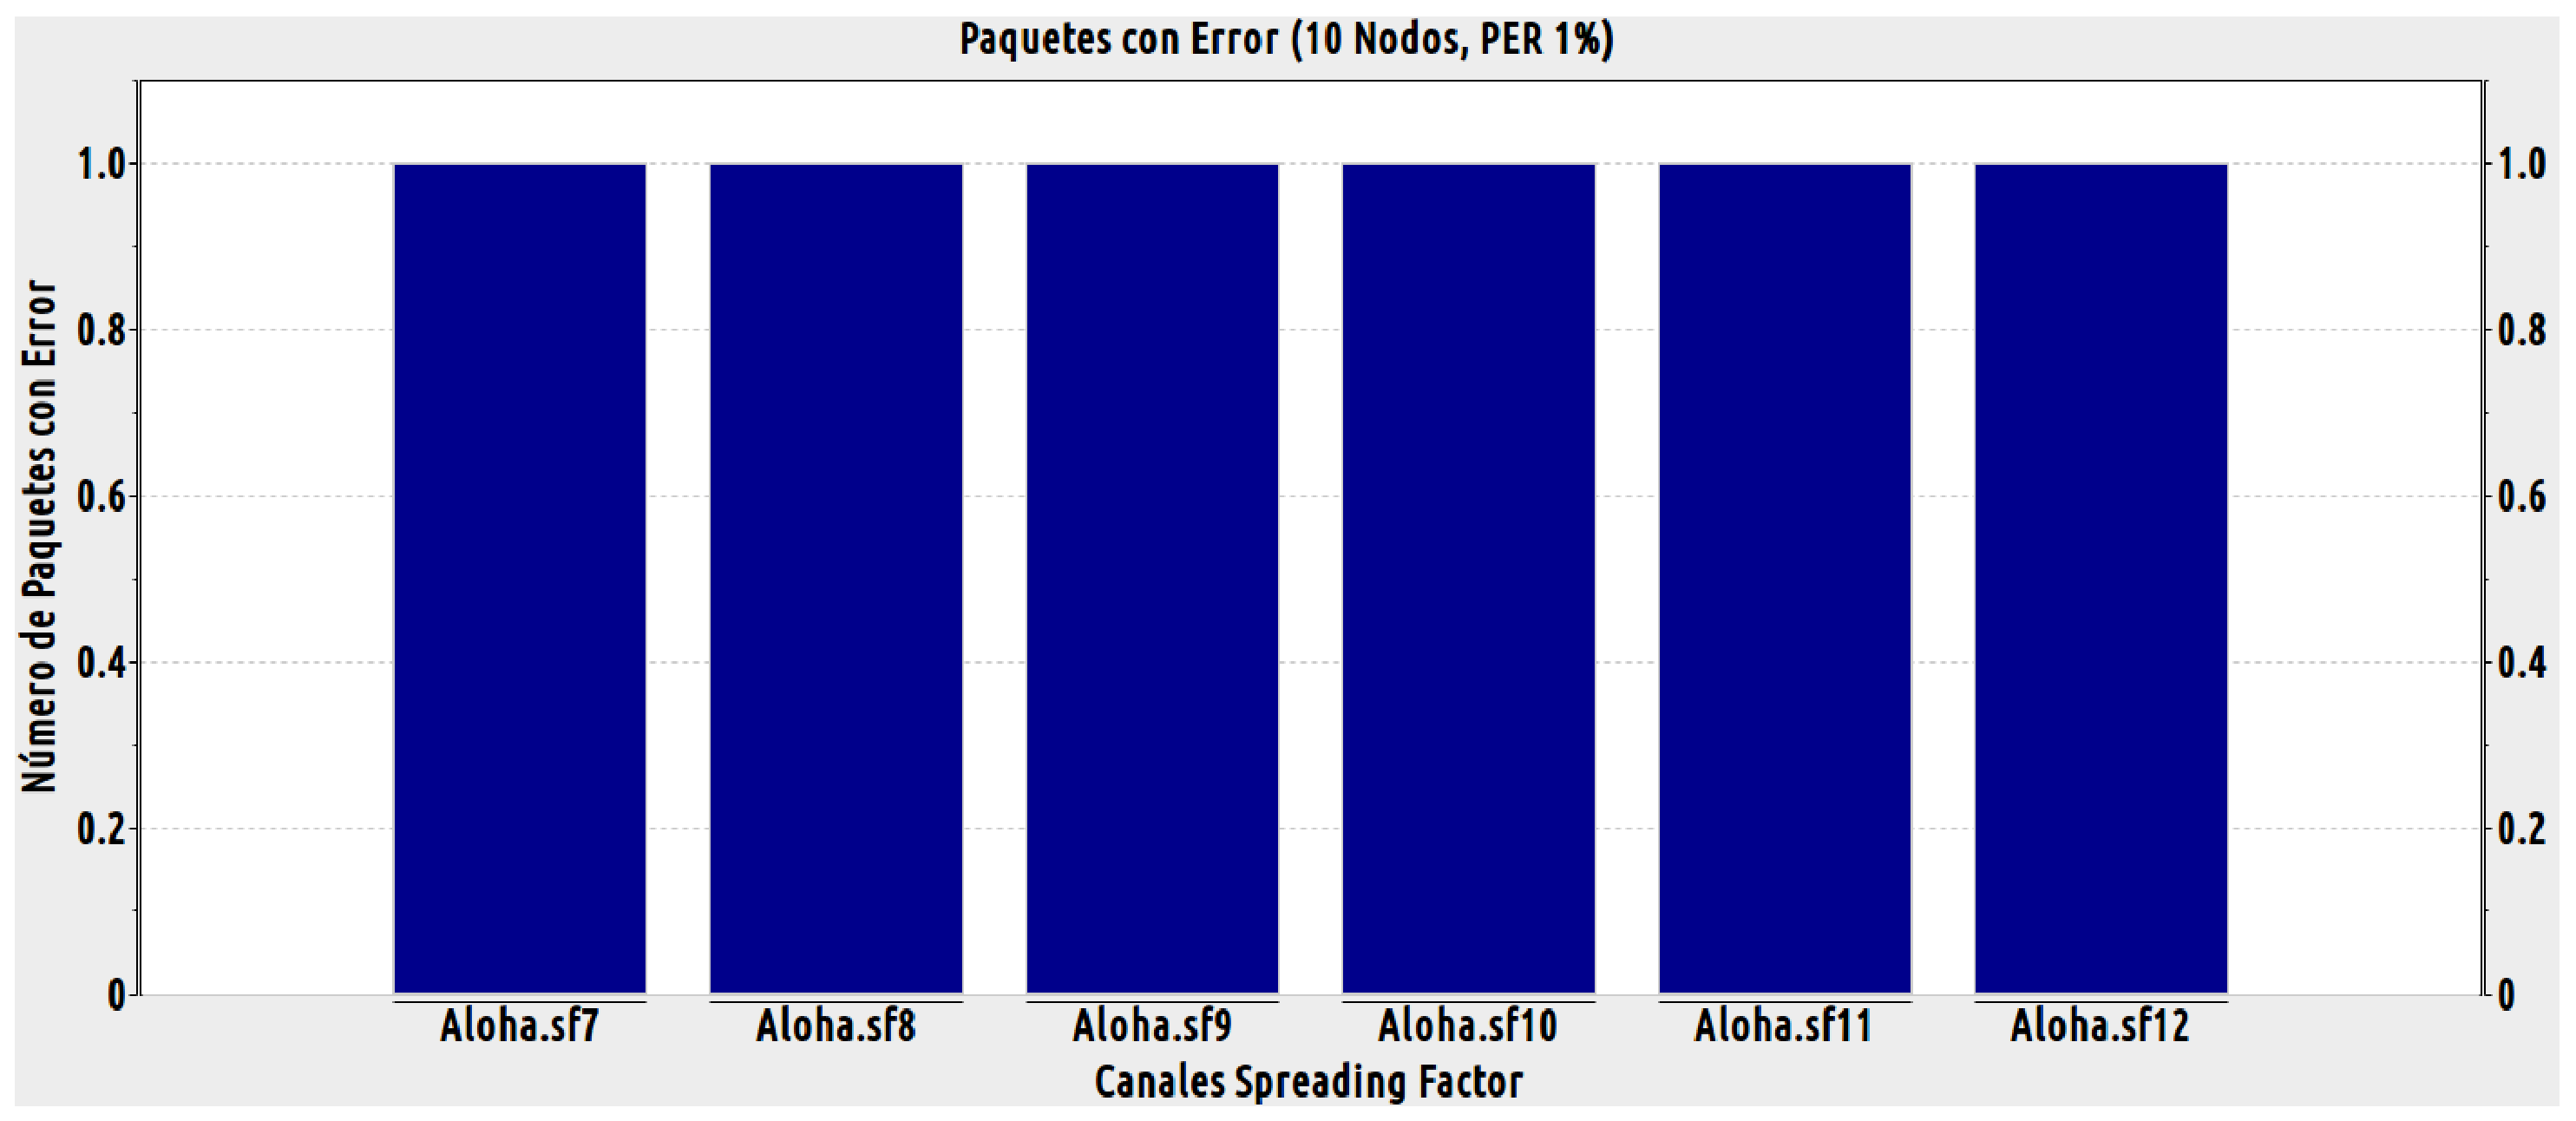
\includegraphics[width=13cm,height=30cm,keepaspectratio]{images/errores10nodos.eps}
\caption{Gráfico de cantidad de paquetes con errores en cada \glsentryname{sf} en la simulación, para 10 nodos. \textit{Esta imagen puede verse ampliada en el Anexo~\ref{anexb:3}}}
\label{prueba:4}
\end{figure}
\noindent
Sin embargo, en la Fig~\ref{prueba:5}, se evidencia un aumento considerable en la cantidad de paquetes con errores, donde la distribución ya no se hace tan homogénea como para el caso de diez nodos. Esto ocurre dado que por las colisiones y el orden arbitrario del simulador \OMNET, donde algunos nodos pertenecientes a determinados \gls{sf} (en este caso particular, el \gls{sf}\num{8}), poseen oportunidades más recurrentes de transmisión que otros, por lo que genera de que algunos \gls{sf} posean una cantidad menor del \SI{1}{\percent}, lo que es esperable, como también que en otros casos, supera el \SI{1}{\percent}. Este evento es debido a que al momento de tomar el estado de la simulación, esta función no terminaba de acomodar el índice de recepción de datos con error al \SI{1}{\percent}, ya que la función que calcula éste índice, a medida que llegan paquetes de forma íntegra al \gls{sf}, este aumenta un contador de envíos recibidos, por lo que al calcular el porcentaje de recepciones con error, este comienza a disminuir de forma paulatina, hasta que disminuye bajo el valor asignado de \gls{per}. Cuando esto ocurre, la función desecha el siguiente paquete en el \gls{sf}, aumentando con esto en uno el contador de recepciones con error y por consecuencia el índice \gls{per}, donde nuevamente sigue calculando de forma cíclica hasta que el porcentaje disminuye hasta el valor asignado al \gls{per}.\newpage \noindent Este evento al no presentarse en todos los \gls{sf} por igual, no se atribuye una falla de diseño, o una falla del simulador, por lo que se presenta como anomalía que depende del tiempo cuando es detenida la simulación al momento de tomar datos estadísticos que representen el comportamiento de los dispositivos.\\
Esta anomalía ocurre de forma análoga para la incongruencia en las colisiones para 100 nodos.
\noindent
\begin{figure}[!ht]
\centering
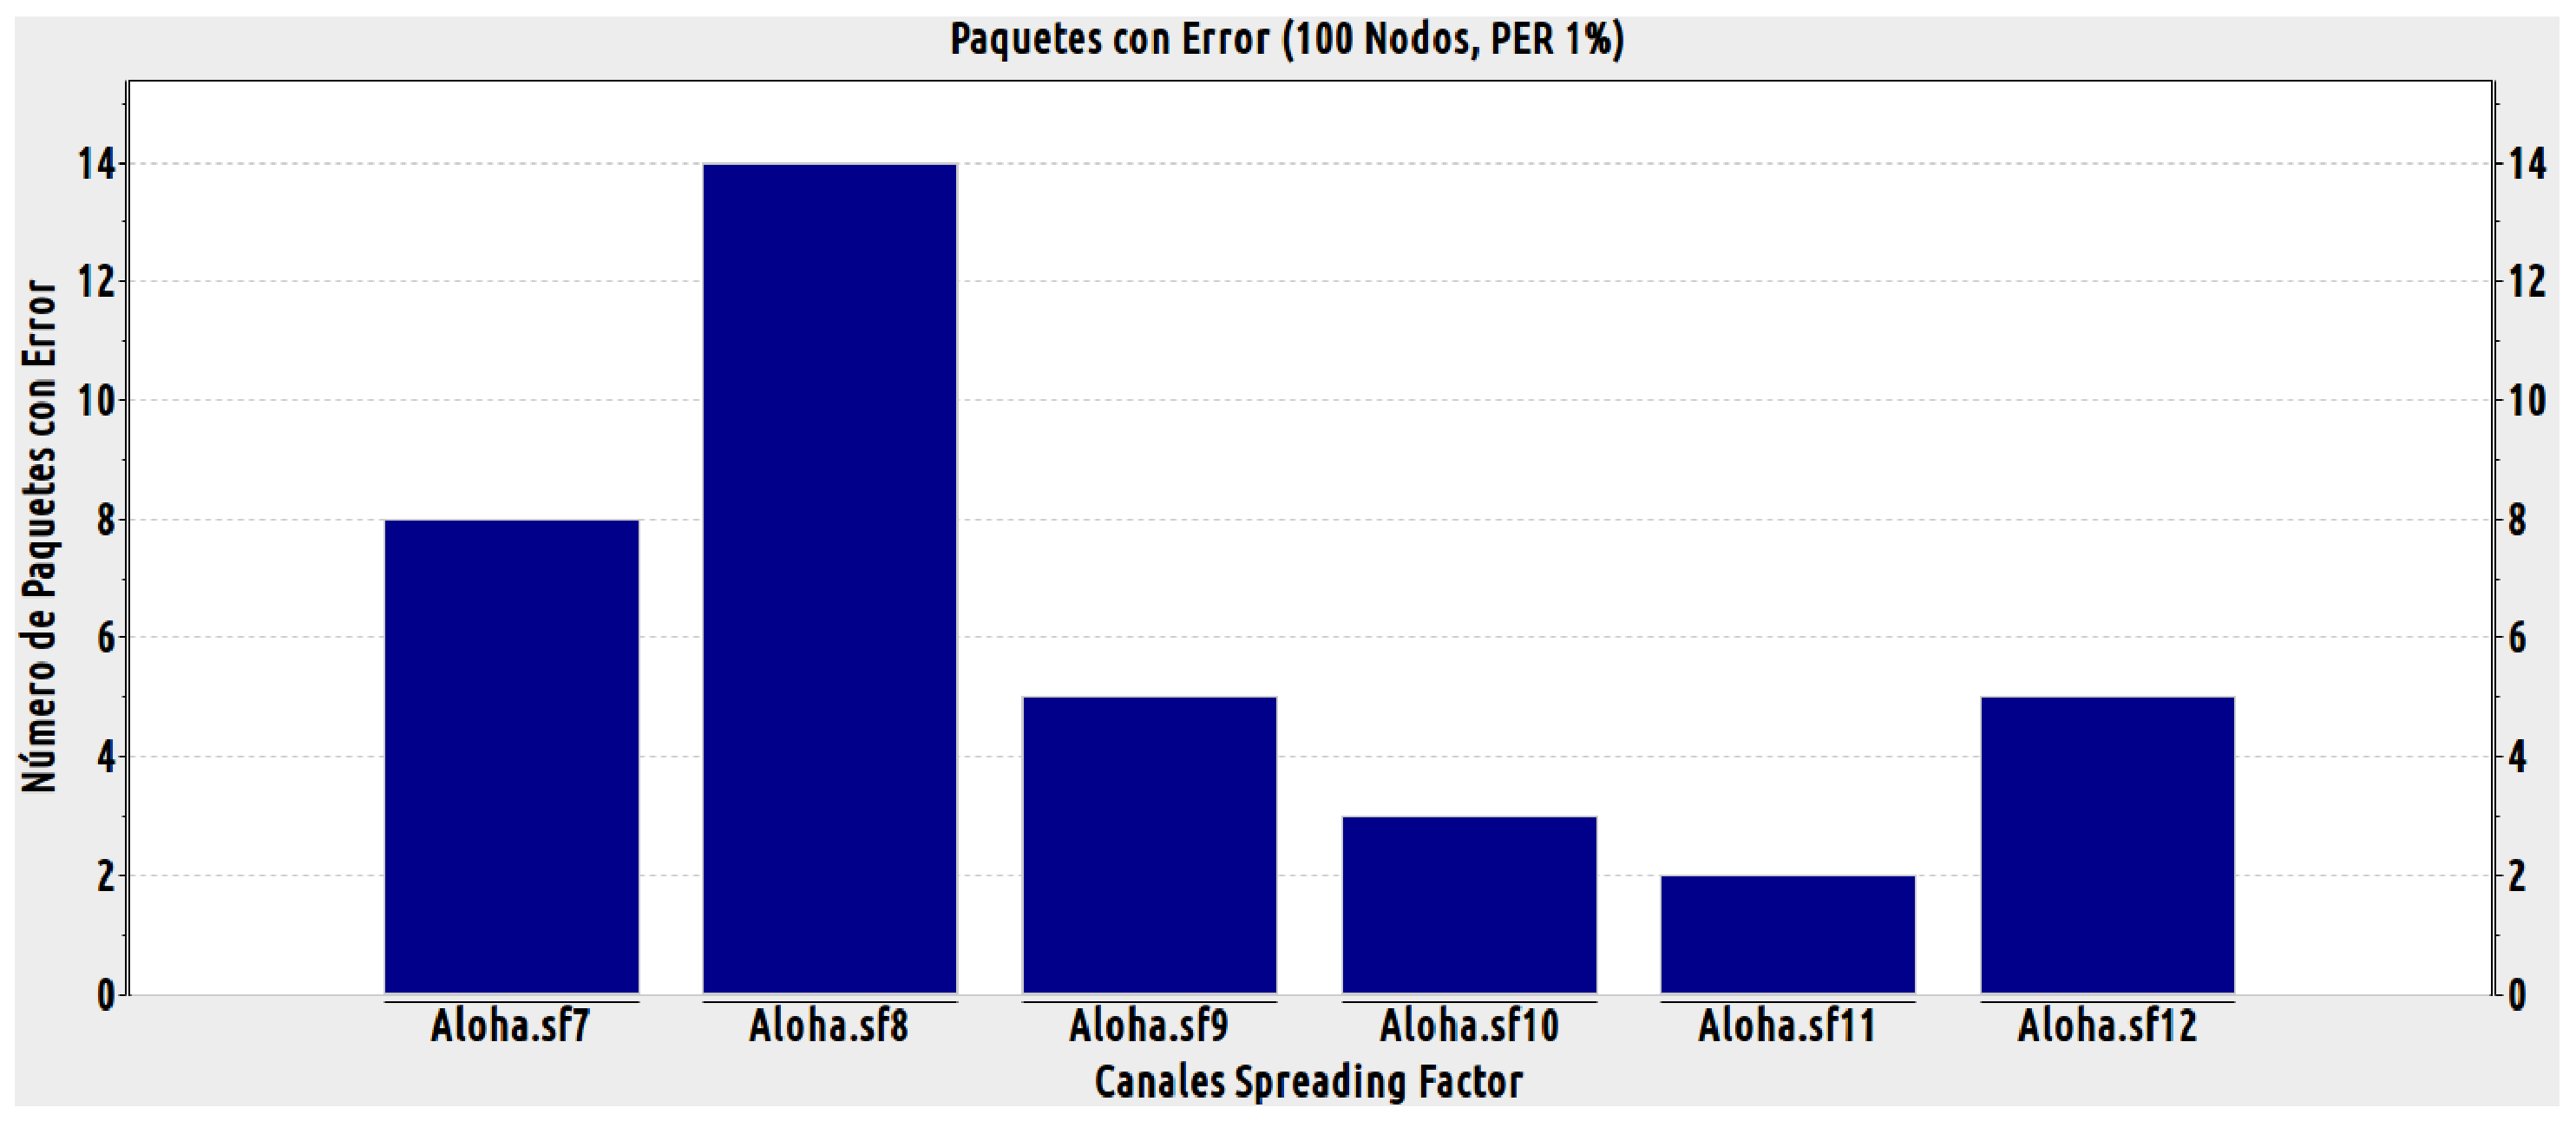
\includegraphics[width=13cm,height=30cm,keepaspectratio]{images/errores100nodos.eps}
\caption{Gráfico de cantidad de paquetes con errores en cada \glsentryname{sf} en la simulación, para 100 nodos. \textit{Esta imagen puede verse ampliada en el Anexo~\ref{anexb:4}}}
\label{prueba:5}
\end{figure}
\end{justify}